%&preformat-disser
\RequirePackage[l2tabu,orthodox]{nag} % Раскомментировав, можно в логе получать рекомендации относительно правильного использования пакетов и предупреждения об устаревших и нерекомендуемых пакетах
% Формат А4, 14pt (ГОСТ Р 7.0.11-2011, 5.3.6)
\documentclass[a4paper,14pt,oneside,openany]{memoir}

%%%%%%%%%%%%%%%%%%%%%%%%%%%%%%%%%%%%%%%%%%%%%%%%%%%%%%
%%%% Файл упрощённых настроек шаблона диссертации %%%%
%%%%%%%%%%%%%%%%%%%%%%%%%%%%%%%%%%%%%%%%%%%%%%%%%%%%%%

%%% Инициализирование переменных, не трогать!  %%%
\newcounter{intvl}
\newcounter{otstup}
\newcounter{contnumeq}
\newcounter{contnumfig}
\newcounter{contnumtab}
\newcounter{pgnum}
\newcounter{chapstyle}
\newcounter{headingdelim}
\newcounter{headingalign}
\newcounter{headingsize}
%%%%%%%%%%%%%%%%%%%%%%%%%%%%%%%%%%%%%%%%%%%%%%%%%%%%%%

%%% Область упрощённого управления оформлением %%%

%% Интервал между заголовками и между заголовком и текстом %%
% Заголовки отделяют от текста сверху и снизу
% тремя интервалами (ГОСТ Р 7.0.11-2011, 5.3.5)
\setcounter{intvl}{1}               % Коэффициент кратности к размеру шрифта

%% Отступы у заголовков в тексте %%
\setcounter{otstup}{0}              % 0 --- без отступа; 1 --- абзацный отступ

%% Нумерация формул, таблиц и рисунков %%
% Нумерация формул
\setcounter{contnumeq}{0}   % 0 --- пораздельно (во введении подряд,
                            %       без номера раздела);
                            % 1 --- сквозная нумерация по всей диссертации
% Нумерация рисунков
\setcounter{contnumfig}{0}  % 0 --- пораздельно (во введении подряд,
                            %       без номера раздела);
                            % 1 --- сквозная нумерация по всей диссертации
% Нумерация таблиц
\setcounter{contnumtab}{1}  % 0 --- пораздельно (во введении подряд,
                            %       без номера раздела);
                            % 1 --- сквозная нумерация по всей диссертации

%% Оглавление %%
\setcounter{pgnum}{1}       % 0 --- номера страниц никак не обозначены;
                            % 1 --- Стр. над номерами страниц (дважды
                            %       компилировать после изменения настройки)
\settocdepth{subsection}    % до какого уровня подразделов выносить в оглавление
\setsecnumdepth{subsection} % до какого уровня нумеровать подразделы


%% Текст и форматирование заголовков %%
\setcounter{chapstyle}{1}     % 0 --- разделы только под номером;
                              % 1 --- разделы с названием "Глава" перед номером
\setcounter{headingdelim}{1}  % 0 --- номер отделен пропуском в 1em или \quad;
                              % 1 --- номера разделов и приложений отделены
                              %       точкой с пробелом, подразделы пропуском
                              %       без точки;
                              % 2 --- номера разделов, подразделов и приложений
                              %       отделены точкой с пробелом.

%% Выравнивание заголовков в тексте %%
\setcounter{headingalign}{0}  % 0 --- по центру;
                              % 1 --- по левому краю

%% Размеры заголовков в тексте %%
\setcounter{headingsize}{0}   % 0 --- по ГОСТ, все всегда 14 пт;
                              % 1 --- пропорционально изменяющийся размер
                              %       в зависимости от базового шрифта

%% Подпись таблиц %%

% Смещение строк подписи после первой строки
\newcommand{\tabindent}{0cm}

% Тип форматирования заголовка таблицы:
% plain --- название и текст в одной строке
% split --- название и текст в разных строках
\newcommand{\tabformat}{plain}

%%% Настройки форматирования таблицы `plain`

% Выравнивание по центру подписи, состоящей из одной строки:
% true  --- выравнивать
% false --- не выравнивать
\newcommand{\tabsinglecenter}{false}

% Выравнивание подписи таблиц:
% justified   --- выравнивать как обычный текст («по ширине»)
% centering   --- выравнивать по центру
% centerlast  --- выравнивать по центру только последнюю строку
% centerfirst --- выравнивать по центру только первую строку (не рекомендуется)
% raggedleft  --- выравнивать по правому краю
% raggedright --- выравнивать по левому краю
\newcommand{\tabjust}{justified}

% Разделитель записи «Таблица #» и названия таблицы
\newcommand{\tablabelsep}{~\cyrdash\ }

%%% Настройки форматирования таблицы `split`

% Положение названия таблицы:
% \centering   --- выравнивать по центру
% \raggedleft  --- выравнивать по правому краю
% \raggedright --- выравнивать по левому краю
\newcommand{\splitformatlabel}{\raggedleft}

% Положение текста подписи:
% \centering   --- выравнивать по центру
% \raggedleft  --- выравнивать по правому краю
% \raggedright --- выравнивать по левому краю
\newcommand{\splitformattext}{\raggedright}

%% Подпись рисунков %%
%Разделитель записи «Рисунок #» и названия рисунка
\newcommand{\figlabelsep}{~\cyrdash\ }  % (ГОСТ 2.105, 4.3.1)
                                        % "--- здесь не работает

%%% Цвета гиперссылок %%%
% Latex color definitions: http://latexcolor.com/
\definecolor{linkcolor}{rgb}{0.9,0,0}
\definecolor{citecolor}{rgb}{0,0.6,0}
\definecolor{urlcolor}{rgb}{0,0,1}
%\definecolor{linkcolor}{rgb}{0,0,0} %black
%\definecolor{citecolor}{rgb}{0,0,0} %black
%\definecolor{urlcolor}{rgb}{0,0,0} %black
            % общие настройки шаблона
%%% Проверка используемого TeX-движка %%%
\newif\ifxetexorluatex   % определяем новый условный оператор (http://tex.stackexchange.com/a/47579)
\ifxetex
    \xetexorluatextrue
\else
    \ifluatex
        \xetexorluatextrue
    \else
        \xetexorluatexfalse
    \fi
\fi

\newif\ifsynopsis           % Условие, проверяющее, что документ --- автореферат

\usepackage{etoolbox}[2015/08/02]   % Для продвинутой проверки разных условий
\providebool{presentation}

\usepackage{comment}    % Позволяет убирать блоки текста (добавляет
                        % окружение comment и команду \excludecomment)

%%% Поля и разметка страницы %%%
\usepackage{pdflscape}  % Для включения альбомных страниц
\usepackage{geometry}   % Для последующего задания полей

%%% Математические пакеты %%%
\usepackage{amsthm,amsmath,amscd}   % Математические дополнения от AMS
\usepackage{amsfonts,amssymb}       % Математические дополнения от AMS
\usepackage{mathtools}              % Добавляет окружение multlined
\usepackage{xfrac}                  % Красивые дроби
\usepackage[
    locale = DE,
    list-separator       = {;\,},
    list-final-separator = {;\,},
    list-pair-separator  = {;\,},
    list-units           = single,
    range-units          = single,
    range-phrase={\text{\ensuremath{-}}},
    % quotient-mode        = fraction, % красивые дроби могут не соответствовать ГОСТ
    fraction-function    = \sfrac,
    separate-uncertainty,
    ]{siunitx}[=v2]                 % Размерности SI
\sisetup{inter-unit-product = \ensuremath{{}\cdot{}}}

% Кириллица в нумерации subequations
% Для правильной работы требуется выполнение сразу после загрузки пакетов
\patchcmd{\subequations}{\def\theequation{\theparentequation\alph{equation}}}
{\def\theequation{\theparentequation\asbuk{equation}}}
{\typeout{subequations patched}}{\typeout{subequations not patched}}

%%%% Установки для размера шрифта 14 pt %%%%
%% Формирование переменных и констант для сравнения (один раз для всех подключаемых файлов)%%
%% должно располагаться до вызова пакета fontspec или polyglossia, потому что они сбивают его работу
\newlength{\curtextsize}
\newlength{\bigtextsize}
\setlength{\bigtextsize}{13.9pt}

\makeatletter
%\show\f@size    % неплохо для отслеживания, но вызывает стопорение процесса,
                 % если документ компилируется без команды  -interaction=nonstopmode
\setlength{\curtextsize}{\f@size pt}
\makeatother

%%% Кодировки и шрифты %%%
\ifxetexorluatex
    \ifpresentation
        \providecommand*\autodot{} % quick fix for polyglossia 1.50
    \fi
    \PassOptionsToPackage{no-math}{fontspec}    % https://tex.stackexchange.com/a/26295/104425
    \usepackage{polyglossia}[2014/05/21]        % Поддержка многоязычности
                                        % (fontspec подгружается автоматически)
\else
   %%% Решение проблемы копирования текста в буфер кракозябрами
    \ifnumequal{\value{usealtfont}}{0}{}{
        \input glyphtounicode.tex
        \input glyphtounicode-cmr.tex %from pdfx package
        \pdfgentounicode=1
    }
    \usepackage{cmap}   % Улучшенный поиск русских слов в полученном pdf-файле
    \ifnumequal{\value{usealtfont}}{2}{}{
        \defaulthyphenchar=127  % Если стоит до fontenc, то переносы
                                % не впишутся в выделяемый текст при
                                % копировании его в буфер обмена
    }
    \usepackage{textcomp}
    \usepackage[T1,T2A]{fontenc}                    % Поддержка русских букв
    \ifnumequal{\value{usealtfont}}{1}{% Используется pscyr, при наличии
        \IfFileExists{pscyr.sty}{\usepackage{pscyr}}{}  % Подключение pscyr
    }{}
    \usepackage[utf8]{inputenc}[2014/04/30]         % Кодировка utf8
    \usepackage[english, russian]{babel}[2014/03/24]% Языки: русский, английский
    \makeatletter\AtBeginDocument{\let\@elt\relax}\makeatother % babel 3.40 fix
    \ifnumequal{\value{usealtfont}}{2}{
        % http://dxdy.ru/post1238763.html#p1238763
        \usepackage[scaled=0.914]{XCharter}[2017/12/19] % Подключение русифицированных шрифтов XCharter
        \usepackage[charter, vvarbb, scaled=1.048]{newtxmath}[2017/12/14]
        \ifpresentation
        \else
            \setDisplayskipStretch{-0.078}
        \fi
    }{}
\fi

%%% Оформление абзацев %%%
\ifpresentation
\else
    \indentafterchapter     % Красная строка после заголовков типа chapter
    \usepackage{indentfirst}
\fi

%%% Цвета %%%
\ifpresentation
\else
    \usepackage[dvipsnames, table, hyperref]{xcolor} % Совместимо с tikz
\fi

%%% Таблицы %%%
\usepackage{longtable} % Длинные таблицы
\usepackage{multirow,makecell}   % Улучшенное форматирование таблиц
\usepackage{tabulary,tabularray} % Таблицы с автоматически подбирающейся
                                 % шириной столбцов
\UseTblrLibrary{booktabs}
\ExplSyntaxOn% define \IfTokenListEmpty to use \captionof with tabularray
\prg_generate_conditional_variant:Nnn \tl_if_empty:n { e } { TF }
\let \IfTokenListEmpty = \tl_if_empty:eTF
\ExplSyntaxOff

\usepackage{threeparttable}      % автоматический подгон ширины подписи таблицы

%%% Общее форматирование
%\usepackage{soul}% Поддержка переносоустойчивых подчёркиваний и зачёркиваний
\usepackage{icomma}  % Запятая в десятичных дробях

%%% Оптимизация расстановки переносов и длины последней строки абзаца
\IfFileExists{impnattypo.sty}{% проверка установленности пакета impnattypo
    \ifluatex
        \ifnumequal{\value{draft}}{1}{% Черновик
            \usepackage[hyphenation, lastparline, nosingleletter, homeoarchy,
            rivers, draft]{impnattypo}
        }{% Чистовик
            \usepackage[hyphenation, lastparline, nosingleletter]{impnattypo}
        }
    \else
        \usepackage[hyphenation, lastparline]{impnattypo}
    \fi
}{}

%% Векторная графика

\usepackage{tikz}                   % Продвинутый пакет векторной графики
\usetikzlibrary{chains}             % Для примера tikz рисунка
\usetikzlibrary{shapes.geometric}   % Для примера tikz рисунка
\usetikzlibrary{shapes.symbols}     % Для примера tikz рисунка
\usetikzlibrary{arrows}             % Для примера tikz рисунка

\usepackage[european,cuteinductors]{circuitikz} % Электрические схемы
\usepackage{pgfplots}                           % Графики
\pgfplotsset{compat=newest}
\usepgfplotslibrary{groupplots,units}
\pgfkeys{/pgf/number format/.cd,use comma,1000 sep={}} % форматирование чисел в графиках

%%% Гиперссылки %%%
\ifxetexorluatex
    \let\CYRDZE\relax
\fi
\usepackage{hyperref}[2012/11/06]

%%% Изображения %%%
\usepackage{graphicx}[2014/04/25]   % Подключаем пакет работы с графикой
\usepackage{caption}                % Подписи рисунков и таблиц
\usepackage{subcaption}             % Подписи подрисунков и подтаблиц
\usepackage{pdfpages}               % Добавление внешних pdf файлов

%%% Счётчики %%%
\usepackage{aliascnt}
\usepackage[figure,table]{totalcount}   % Счётчик рисунков и таблиц
\usepackage{totcount}   % Пакет создания счётчиков на основе последнего номера
                        % подсчитываемого элемента (может требовать дважды
                        % компилировать документ)
\usepackage{totpages}   % Счётчик страниц, совместимый с hyperref (ссылается
                        % на номер последней страницы). Желательно ставить
                        % последним пакетом в преамбуле

%%% Продвинутое управление групповыми ссылками (пока только формулами) %%%
\ifpresentation
\else
    \usepackage[russian]{cleveref} % cleveref имеет сложности со считыванием
    % языка из babel. Такое решение русификации вывода выбрано вместо
    % определения в documentclass из опасности что-то лишнее передать во все
    % остальные пакеты, включая библиографию.

    % Добавление возможности использования пробелов в \labelcref
    % https://tex.stackexchange.com/a/340502/104425
    \usepackage{kvsetkeys}
    \makeatletter
    \let\org@@cref\@cref
    \renewcommand*{\@cref}[2]{%
        \edef\process@me{%
            \noexpand\org@@cref{#1}{\zap@space#2 \@empty}%
        }\process@me
    }
    \makeatother
\fi

\usepackage{placeins} % для \FloatBarrier

\ifnumequal{\value{draft}}{1}{% Черновик
    \usepackage[firstpage]{draftwatermark}
    \SetWatermarkText{DRAFT}
    \SetWatermarkFontSize{14pt}
    \SetWatermarkScale{15}
    \SetWatermarkAngle{45}
}{}

%%% Цитата, не приводимая в автореферате:
% возможно, актуальна только для biblatex
%\newcommand{\citeinsynopsis}[1]{\ifsynopsis\else ~\cite{#1} \fi}

% если текущий процесс запущен библиотекой tikz-external, то прекомпиляция должна быть включена
\ifdefined\tikzexternalrealjob
    \setcounter{imgprecompile}{1}
\fi

\ifnumequal{\value{imgprecompile}}{1}{% Только если у нас включена предкомпиляция
    \usetikzlibrary{external}   % подключение возможности предкомпиляции
    \tikzexternalize[prefix=images/cache/,optimize command away=\includepdf] % activate! % здесь можно указать отдельную папку для скомпилированных файлов
    \ifxetex
        \tikzset{external/up to date check={diff}}
    \fi
}{}
         % Пакеты общие для диссертации и автореферата
\synopsisfalse                      % Этот документ --- не автореферат
\input{Dissertation/dispackages}    % Пакеты для диссертации
\input{Dissertation/userpackages}   % Пакеты для специфических пользовательских задач

%%%%%%%%%%%%%%%%%%%%%%%%%%%%%%%%%%%%%%%%%%%%%%%%%%%%%%
%%%% Файл упрощённых настроек шаблона диссертации %%%%
%%%%%%%%%%%%%%%%%%%%%%%%%%%%%%%%%%%%%%%%%%%%%%%%%%%%%%

%%% Инициализирование переменных, не трогать!  %%%
\newcounter{intvl}
\newcounter{otstup}
\newcounter{contnumeq}
\newcounter{contnumfig}
\newcounter{contnumtab}
\newcounter{pgnum}
\newcounter{chapstyle}
\newcounter{headingdelim}
\newcounter{headingalign}
\newcounter{headingsize}
%%%%%%%%%%%%%%%%%%%%%%%%%%%%%%%%%%%%%%%%%%%%%%%%%%%%%%

%%% Область упрощённого управления оформлением %%%

%% Интервал между заголовками и между заголовком и текстом %%
% Заголовки отделяют от текста сверху и снизу
% тремя интервалами (ГОСТ Р 7.0.11-2011, 5.3.5)
\setcounter{intvl}{1}               % Коэффициент кратности к размеру шрифта

%% Отступы у заголовков в тексте %%
\setcounter{otstup}{0}              % 0 --- без отступа; 1 --- абзацный отступ

%% Нумерация формул, таблиц и рисунков %%
% Нумерация формул
\setcounter{contnumeq}{0}   % 0 --- пораздельно (во введении подряд,
                            %       без номера раздела);
                            % 1 --- сквозная нумерация по всей диссертации
% Нумерация рисунков
\setcounter{contnumfig}{0}  % 0 --- пораздельно (во введении подряд,
                            %       без номера раздела);
                            % 1 --- сквозная нумерация по всей диссертации
% Нумерация таблиц
\setcounter{contnumtab}{1}  % 0 --- пораздельно (во введении подряд,
                            %       без номера раздела);
                            % 1 --- сквозная нумерация по всей диссертации

%% Оглавление %%
\setcounter{pgnum}{1}       % 0 --- номера страниц никак не обозначены;
                            % 1 --- Стр. над номерами страниц (дважды
                            %       компилировать после изменения настройки)
\settocdepth{subsection}    % до какого уровня подразделов выносить в оглавление
\setsecnumdepth{subsection} % до какого уровня нумеровать подразделы


%% Текст и форматирование заголовков %%
\setcounter{chapstyle}{1}     % 0 --- разделы только под номером;
                              % 1 --- разделы с названием "Глава" перед номером
\setcounter{headingdelim}{1}  % 0 --- номер отделен пропуском в 1em или \quad;
                              % 1 --- номера разделов и приложений отделены
                              %       точкой с пробелом, подразделы пропуском
                              %       без точки;
                              % 2 --- номера разделов, подразделов и приложений
                              %       отделены точкой с пробелом.

%% Выравнивание заголовков в тексте %%
\setcounter{headingalign}{0}  % 0 --- по центру;
                              % 1 --- по левому краю

%% Размеры заголовков в тексте %%
\setcounter{headingsize}{0}   % 0 --- по ГОСТ, все всегда 14 пт;
                              % 1 --- пропорционально изменяющийся размер
                              %       в зависимости от базового шрифта

%% Подпись таблиц %%

% Смещение строк подписи после первой строки
\newcommand{\tabindent}{0cm}

% Тип форматирования заголовка таблицы:
% plain --- название и текст в одной строке
% split --- название и текст в разных строках
\newcommand{\tabformat}{plain}

%%% Настройки форматирования таблицы `plain`

% Выравнивание по центру подписи, состоящей из одной строки:
% true  --- выравнивать
% false --- не выравнивать
\newcommand{\tabsinglecenter}{false}

% Выравнивание подписи таблиц:
% justified   --- выравнивать как обычный текст («по ширине»)
% centering   --- выравнивать по центру
% centerlast  --- выравнивать по центру только последнюю строку
% centerfirst --- выравнивать по центру только первую строку (не рекомендуется)
% raggedleft  --- выравнивать по правому краю
% raggedright --- выравнивать по левому краю
\newcommand{\tabjust}{justified}

% Разделитель записи «Таблица #» и названия таблицы
\newcommand{\tablabelsep}{~\cyrdash\ }

%%% Настройки форматирования таблицы `split`

% Положение названия таблицы:
% \centering   --- выравнивать по центру
% \raggedleft  --- выравнивать по правому краю
% \raggedright --- выравнивать по левому краю
\newcommand{\splitformatlabel}{\raggedleft}

% Положение текста подписи:
% \centering   --- выравнивать по центру
% \raggedleft  --- выравнивать по правому краю
% \raggedright --- выравнивать по левому краю
\newcommand{\splitformattext}{\raggedright}

%% Подпись рисунков %%
%Разделитель записи «Рисунок #» и названия рисунка
\newcommand{\figlabelsep}{~\cyrdash\ }  % (ГОСТ 2.105, 4.3.1)
                                        % "--- здесь не работает

%%% Цвета гиперссылок %%%
% Latex color definitions: http://latexcolor.com/
\definecolor{linkcolor}{rgb}{0.9,0,0}
\definecolor{citecolor}{rgb}{0,0.6,0}
\definecolor{urlcolor}{rgb}{0,0,1}
%\definecolor{linkcolor}{rgb}{0,0,0} %black
%\definecolor{citecolor}{rgb}{0,0,0} %black
%\definecolor{urlcolor}{rgb}{0,0,0} %black
      % Упрощённые настройки шаблона

\input{common/newnames}         % Новые переменные, для всего проекта

%%% Основные сведения %%%
\newcommand{\thesisAuthorLastName}{Соловьев}
\newcommand{\thesisAuthorOtherNames}{Виктор Владимирович}
\newcommand{\thesisAuthorInitials}{В.\,В.}
\newcommand{\thesisAuthor}             % Диссертация, ФИО автора
{%
    \texorpdfstring{% \texorpdfstring takes two arguments and uses the first for (La)TeX and the second for pdf
        \thesisAuthorLastName~\thesisAuthorOtherNames% так будет отображаться на титульном листе или в тексте, где будет использоваться переменная
    }{%
        \thesisAuthorLastName, \thesisAuthorOtherNames% эта запись для свойств pdf-файла. В таком виде, если pdf будет обработан программами для сбора библиографических сведений, будет правильно представлена фамилия.
    }
}
\newcommand{\thesisAuthorShort}        % Диссертация, ФИО автора инициалами
{\thesisAuthorInitials~\thesisAuthorLastName}
%\newcommand{\thesisUdk}                % Диссертация, УДК
%{\fixme{xxx.xxx}}
\newcommand{\thesisTitle}              % Диссертация, название
{Математическое моделирование и~разработка методов автоматизации рабочих процессов наземных
транспортно-технологических средств}
\newcommand{\thesisSpecialtyNumber}    % Диссертация, специальность, номер
{5.2.11}
\newcommand{\thesisSpecialtyTitle}     % Диссертация, специальность, название (название взято с сайта ВАК для примера)
{Наземные транспортно-технологические средства и~комплексы}
%% \newcommand{\thesisSpecialtyTwoNumber} % Диссертация, вторая специальность, номер
%% {\fixme{XX.XX.XX}}
%% \newcommand{\thesisSpecialtyTwoTitle}  % Диссертация, вторая специальность, название
%% {\fixme{Теория и~методика физического воспитания, спортивной тренировки,
%% оздоровительной и~адаптивной физической культуры}}
\newcommand{\thesisDegree}             % Диссертация, ученая степень
{кандидата технических наук}
\newcommand{\thesisDegreeShort}        % Диссертация, ученая степень, краткая запись
{канд. техн. наук}
\newcommand{\thesisCity}               % Диссертация, город написания диссертации
{Санкт-Петербург}
\newcommand{\thesisYear}               % Диссертация, год написания диссертации
{\the\year}
\newcommand{\thesisOrganization}       % Диссертация, организация
{Федеральное государственное бюджетное образовательное учреждение высшего
образования <<Санкт-Петербургский государственный архитектурно-строительный университет <<СПб ГАСУ>>}
\newcommand{\thesisOrganizationShort}  % Диссертация, краткое название организации для доклада
{Матмоделирование и~разработка методов автоматизации рабочих процессов НТТС}

\newcommand{\thesisInOrganization}     % Диссертация, организация в предложном падеже: Работа выполнена в ...
{федеральном государственном бюджетном образовательном учреждении высшего образования <<Санкт-Петербургский государственный архитектурно-строительный университет <<СПб ГАСУ>>}

%% \newcommand{\supervisorDead}{}           % Рисовать рамку вокруг фамилии
\newcommand{\supervisorFio}              % Научный руководитель, ФИО
{Евтюков Сергей Аркадьевич}
\newcommand{\supervisorRegalia}          % Научный руководитель, регалии
{доктор технических наук, профессор}
\newcommand{\supervisorFioShort}         % Научный руководитель, ФИО
{С.\,А.~Евтюков}
\newcommand{\supervisorRegaliaShort}     % Научный руководитель, регалии
{д.т.н.,~проф.}

%% \newcommand{\supervisorTwoDead}{}        % Рисовать рамку вокруг фамилии
%% \newcommand{\supervisorTwoFio}           % Второй научный руководитель, ФИО
%% {\fixme{Фамилия Имя Отчество}}
%% \newcommand{\supervisorTwoRegalia}       % Второй научный руководитель, регалии
%% {\fixme{уч. степень, уч. звание}}
%% \newcommand{\supervisorTwoFioShort}      % Второй научный руководитель, ФИО
%% {\fixme{И.\,О.~Фамилия}}
%% \newcommand{\supervisorTwoRegaliaShort}  % Второй научный руководитель, регалии
%% {\fixme{уч.~ст.,~уч.~зв.}}

\newcommand{\opponentOneFio}           % Оппонент 1, ФИО
{\fixme{Фамилия Имя Отчество}}
\newcommand{\opponentOneRegalia}       % Оппонент 1, регалии
{\fixme{доктор физико-математических наук, профессор}}
\newcommand{\opponentOneJobPlace}      % Оппонент 1, место работы
{\fixme{Не очень длинное название для места работы}}
\newcommand{\opponentOneJobPost}       % Оппонент 1, должность
{\fixme{старший научный сотрудник}}

\newcommand{\opponentTwoFio}           % Оппонент 2, ФИО
{\fixme{Фамилия Имя Отчество}}
\newcommand{\opponentTwoRegalia}       % Оппонент 2, регалии
{\fixme{кандидат физико-математических наук}}
\newcommand{\opponentTwoJobPlace}      % Оппонент 2, место работы
{\fixme{Основное место работы c длинным длинным длинным длинным названием}}
\newcommand{\opponentTwoJobPost}       % Оппонент 2, должность
{\fixme{старший научный сотрудник}}

%% \newcommand{\opponentThreeFio}         % Оппонент 3, ФИО
%% {\fixme{Фамилия Имя Отчество}}
%% \newcommand{\opponentThreeRegalia}     % Оппонент 3, регалии
%% {\fixme{кандидат физико-математических наук}}
%% \newcommand{\opponentThreeJobPlace}    % Оппонент 3, место работы
%% {\fixme{Основное место работы c длинным длинным длинным длинным названием}}
%% \newcommand{\opponentThreeJobPost}     % Оппонент 3, должность
%% {\fixme{старший научный сотрудник}}

\newcommand{\leadingOrganizationTitle} % Ведущая организация, дополнительные строки. Удалить, чтобы не отображать в автореферате
{\fixme{Федеральное государственное бюджетное образовательное учреждение высшего
профессионального образования с~длинным длинным длинным длинным названием}}

\newcommand{\defenseDate}              % Защита, дата
{\fixme{DD mmmmmmmm YYYY~г.~в~XX часов}}
\newcommand{\defenseCouncilNumber}     % Защита, номер диссертационного совета
{\fixme{Д\,123.456.78}}
\newcommand{\defenseCouncilTitle}      % Защита, учреждение диссертационного совета
{\fixme{Название учреждения}}
\newcommand{\defenseCouncilAddress}    % Защита, адрес учреждение диссертационного совета
{\fixme{Адрес}}
\newcommand{\defenseCouncilPhone}      % Телефон для справок
{\fixme{+7~(0000)~00-00-00}}

\newcommand{\defenseSecretaryFio}      % Секретарь диссертационного совета, ФИО
{\fixme{Фамилия Имя Отчество}}
\newcommand{\defenseSecretaryRegalia}  % Секретарь диссертационного совета, регалии
{\fixme{д-р~физ.-мат. наук}}            % Для сокращений есть ГОСТы, например: ГОСТ Р 7.0.12-2011 + http://base.garant.ru/179724/#block_30000

\newcommand{\synopsisLibrary}          % Автореферат, название библиотеки
{\fixme{Название библиотеки}}
\newcommand{\synopsisDate}             % Автореферат, дата рассылки
{\fixme{DD mmmmmmmm}\the\year~года}

% To avoid conflict with beamer class use \providecommand
\providecommand{\keywords}%            % Ключевые слова для метаданных PDF диссертации и автореферата
{}
             % Основные сведения
%%% Кодировки и шрифты %%%
\ifxetexorluatex
    % Язык по-умолчанию русский с поддержкой приятных команд пакета babel
    \setmainlanguage[babelshorthands=true]{russian}
    % Дополнительный язык = английский (в американской вариации по-умолчанию)
    \setotherlanguage{english}

    % Проверка существования шрифтов. Недоступна в pdflatex
    \ifnumequal{\value{fontfamily}}{1}{
        \IfFontExistsTF{Times New Roman}{}{\setcounter{fontfamily}{0}}
    }{}
    \ifnumequal{\value{fontfamily}}{2}{
        \IfFontExistsTF{LiberationSerif}{}{\setcounter{fontfamily}{0}}
    }{}

    \ifnumequal{\value{fontfamily}}{0}{% Семейство шрифтов CMU. Используется как fallback
        \setmonofont[
          BoldFont={cmuntb.otf},
          ItalicFont={cmunit.otf},
          BoldItalicFont={cmuntx.otf}
        ]{cmuntt.otf} % {CMU Typewriter Text} % моноширинный шрифт
        \newfontfamily\cyrillicfonttt[
          BoldFont={cmuntb.otf},
          ItalicFont={cmunit.otf},
          BoldItalicFont={cmuntx.otf}
        ]{cmuntt.otf} % {CMU Typewriter Text} % моноширинный шрифт для кириллицы
        \defaultfontfeatures{Ligatures=TeX}   % стандартные лигатуры TeX, замены нескольких дефисов на тире и т. п. Настройки моноширинного шрифта должны идти до этой строки, чтобы при врезках кода программ в коде не применялись лигатуры и замены дефисов
        \setmainfont[
          SlantedFont={cmunsl.otf},
          BoldSlantedFont={cmunbl.otf},
          BoldFont={cmunbx.otf},
          ItalicFont={cmunti.otf},
          BoldItalicFont={cmunbi.otf}
        ]{cmunrm.otf} % {CMU Serif}           % Шрифт с засечками
        \newfontfamily\cyrillicfont[
          SlantedFont={cmunsl.otf},
          BoldSlantedFont={cmunbl.otf},
          BoldFont={cmunbx.otf},
          ItalicFont={cmunti.otf},
          BoldItalicFont={cmunbi.otf}
        ]{cmunrm.otf}   % {CMU Serif}         % Шрифт с засечками для кириллицы
        \setsansfont[
          BoldFont={cmunsx.otf},
          ItalicFont={cmunsi.otf},
          BoldItalicFont={cmunso.otf}
        ]{cmunss.otf} % {CMU Sans Serif}      % Шрифт без засечек
        \newfontfamily\cyrillicfontsf[
          BoldFont={cmunsx.otf},
          ItalicFont={cmunsi.otf},
          BoldItalicFont={cmunso.otf}
        ]{cmunss.otf} % {CMU Sans Serif}      % Шрифт без засечек для кириллицы
    }

    \ifnumequal{\value{fontfamily}}{1}{                    % Семейство MS шрифтов
        \setmonofont{Courier New}                          % моноширинный шрифт
        \newfontfamily\cyrillicfonttt{Courier New}         % моноширинный шрифт для кириллицы
        \defaultfontfeatures{Ligatures=TeX}                % стандартные лигатуры TeX, замены нескольких дефисов на тире и т. п. Настройки моноширинного шрифта должны идти до этой строки, чтобы при врезках кода программ в коде не применялись лигатуры и замены дефисов
        \setmainfont{Times New Roman}                      % Шрифт с засечками
        \newfontfamily\cyrillicfont{Times New Roman}       % Шрифт с засечками для кириллицы
        \setsansfont{Arial}                                % Шрифт без засечек
        \newfontfamily\cyrillicfontsf{Arial}               % Шрифт без засечек для кириллицы
    }

    \ifnumequal{\value{fontfamily}}{2}{                    % Семейство шрифтов Liberation (https://pagure.io/liberation-fonts)
        \setmonofont{LiberationMono}[Scale=0.87] % моноширинный шрифт
        \newfontfamily\cyrillicfonttt{LiberationMono}[     % моноширинный шрифт для кириллицы
            Scale=0.87]
        \defaultfontfeatures{Ligatures=TeX}                % стандартные лигатуры TeX, замены нескольких дефисов на тире и т. п. Настройки моноширинного шрифта должны идти до этой строки, чтобы при врезках кода программ в коде не применялись лигатуры и замены дефисов
        \setmainfont{LiberationSerif}                      % Шрифт с засечками
        \newfontfamily\cyrillicfont{LiberationSerif}       % Шрифт с засечками для кириллицы
        \setsansfont{LiberationSans}                       % Шрифт без засечек
        \newfontfamily\cyrillicfontsf{LiberationSans}      % Шрифт без засечек для кириллицы
    }

\else
    \ifnumequal{\value{usealtfont}}{1}{% Используется pscyr, при наличии
        \IfFileExists{pscyr.sty}{\renewcommand{\rmdefault}{ftm}}{}
    }{}
\fi
            % Определение шрифтов (частичное)
\input{common/styles}           % Стили общие для диссертации и автореферата
\input{Dissertation/disstyles}  % Стили для диссертации
% для вертикального центрирования ячеек в tabulary
\def\zz{\ifx\[$\else\aftergroup\zzz\fi}
%$ \] % <-- чиним подсветку синтаксиса в некоторых редакторах
\def\zzz{\setbox0\lastbox
\dimen0\dimexpr\extrarowheight + \ht0-\dp0\relax
\setbox0\hbox{\raise-.5\dimen0\box0}%
\ht0=\dimexpr\ht0+\extrarowheight\relax
\dp0=\dimexpr\dp0+\extrarowheight\relax
\box0
}

\lstdefinelanguage{Renhanced}%
{keywords={abbreviate,abline,abs,acos,acosh,action,add1,add,%
        aggregate,alias,Alias,alist,all,anova,any,aov,aperm,append,apply,%
        approx,approxfun,apropos,Arg,args,array,arrows,as,asin,asinh,%
        atan,atan2,atanh,attach,attr,attributes,autoload,autoloader,ave,%
        axis,backsolve,barplot,basename,besselI,besselJ,besselK,besselY,%
        beta,binomial,body,box,boxplot,break,browser,bug,builtins,bxp,by,%
        c,C,call,Call,case,cat,category,cbind,ceiling,character,char,%
        charmatch,check,chol,chol2inv,choose,chull,class,close,cm,codes,%
        coef,coefficients,co,col,colnames,colors,colours,commandArgs,%
        comment,complete,complex,conflicts,Conj,contents,contour,%
        contrasts,contr,control,helmert,contrib,convolve,cooks,coords,%
        distance,coplot,cor,cos,cosh,count,fields,cov,covratio,wt,CRAN,%
        create,crossprod,cummax,cummin,cumprod,cumsum,curve,cut,cycle,D,%
        data,dataentry,date,dbeta,dbinom,dcauchy,dchisq,de,debug,%
        debugger,Defunct,default,delay,delete,deltat,demo,de,density,%
        deparse,dependencies,Deprecated,deriv,description,detach,%
        dev2bitmap,dev,cur,deviance,off,prev,,dexp,df,dfbetas,dffits,%
        dgamma,dgeom,dget,dhyper,diag,diff,digamma,dim,dimnames,dir,%
        dirname,dlnorm,dlogis,dnbinom,dnchisq,dnorm,do,dotplot,double,%
        download,dpois,dput,drop,drop1,dsignrank,dt,dummy,dump,dunif,%
        duplicated,dweibull,dwilcox,dyn,edit,eff,effects,eigen,else,%
        emacs,end,environment,env,erase,eval,equal,evalq,example,exists,%
        exit,exp,expand,expression,External,extract,extractAIC,factor,%
        fail,family,fft,file,filled,find,fitted,fivenum,fix,floor,for,%
        For,formals,format,formatC,formula,Fortran,forwardsolve,frame,%
        frequency,ftable,ftable2table,function,gamma,Gamma,gammaCody,%
        gaussian,gc,gcinfo,gctorture,get,getenv,geterrmessage,getOption,%
        getwd,gl,glm,globalenv,gnome,GNOME,graphics,gray,grep,grey,grid,%
        gsub,hasTsp,hat,heat,help,hist,home,hsv,httpclient,I,identify,if,%
        ifelse,Im,image,\%in\%,index,influence,measures,inherits,install,%
        installed,integer,interaction,interactive,Internal,intersect,%
        inverse,invisible,IQR,is,jitter,kappa,kronecker,labels,lapply,%
        layout,lbeta,lchoose,lcm,legend,length,levels,lgamma,library,%
        licence,license,lines,list,lm,load,local,locator,log,log10,log1p,%
        log2,logical,loglin,lower,lowess,ls,lsfit,lsf,ls,machine,Machine,%
        mad,mahalanobis,make,link,margin,match,Math,matlines,mat,matplot,%
        matpoints,matrix,max,mean,median,memory,menu,merge,methods,min,%
        missing,Mod,mode,model,response,mosaicplot,mtext,mvfft,na,nan,%
        names,omit,nargs,nchar,ncol,NCOL,new,next,NextMethod,nextn,%
        nlevels,nlm,noquote,NotYetImplemented,NotYetUsed,nrow,NROW,null,%
        numeric,\%o\%,objects,offset,old,on,Ops,optim,optimise,optimize,%
        options,or,order,ordered,outer,package,packages,page,pairlist,%
        pairs,palette,panel,par,parent,parse,paste,path,pbeta,pbinom,%
        pcauchy,pchisq,pentagamma,persp,pexp,pf,pgamma,pgeom,phyper,pico,%
        pictex,piechart,Platform,plnorm,plogis,plot,pmatch,pmax,pmin,%
        pnbinom,pnchisq,pnorm,points,poisson,poly,polygon,polyroot,pos,%
        postscript,power,ppoints,ppois,predict,preplot,pretty,Primitive,%
        print,prmatrix,proc,prod,profile,proj,prompt,prop,provide,%
        psignrank,ps,pt,ptukey,punif,pweibull,pwilcox,q,qbeta,qbinom,%
        qcauchy,qchisq,qexp,qf,qgamma,qgeom,qhyper,qlnorm,qlogis,qnbinom,%
        qnchisq,qnorm,qpois,qqline,qqnorm,qqplot,qr,Q,qty,qy,qsignrank,%
        qt,qtukey,quantile,quasi,quit,qunif,quote,qweibull,qwilcox,%
        rainbow,range,rank,rbeta,rbind,rbinom,rcauchy,rchisq,Re,read,csv,%
        csv2,fwf,readline,socket,real,Recall,rect,reformulate,regexpr,%
        relevel,remove,rep,repeat,replace,replications,report,require,%
        resid,residuals,restart,return,rev,rexp,rf,rgamma,rgb,rgeom,R,%
        rhyper,rle,rlnorm,rlogis,rm,rnbinom,RNGkind,rnorm,round,row,%
        rownames,rowsum,rpois,rsignrank,rstandard,rstudent,rt,rug,runif,%
        rweibull,rwilcox,sample,sapply,save,scale,scan,scan,screen,sd,se,%
        search,searchpaths,segments,seq,sequence,setdiff,setequal,set,%
        setwd,show,sign,signif,sin,single,sinh,sink,solve,sort,source,%
        spline,splinefun,split,sqrt,stars,start,stat,stem,step,stop,%
        storage,strstrheight,stripplot,strsplit,structure,strwidth,sub,%
        subset,substitute,substr,substring,sum,summary,sunflowerplot,svd,%
        sweep,switch,symbol,symbols,symnum,sys,status,system,t,table,%
        tabulate,tan,tanh,tapply,tempfile,terms,terrain,tetragamma,text,%
        time,title,topo,trace,traceback,transform,tri,trigamma,trunc,try,%
        ts,tsp,typeof,unclass,undebug,undoc,union,unique,uniroot,unix,%
        unlink,unlist,unname,untrace,update,upper,url,UseMethod,var,%
        variable,vector,Version,vi,warning,warnings,weighted,weights,%
        which,while,window,write,\%x\%,x11,X11,xedit,xemacs,xinch,xor,%
        xpdrows,xy,xyinch,yinch,zapsmall,zip},%
    otherkeywords={!,!=,~,$,*,\%,\&,\%/\%,\%*\%,\%\%,<-,<<-},%$
    alsoother={._$},%$
    sensitive,%
    morecomment=[l]\#,%
    morestring=[d]",%
    morestring=[d]'% 2001 Robert Denham
}%

%решаем проблему с кириллицей в комментариях (в pdflatex) https://tex.stackexchange.com/a/103712
\lstset{extendedchars=true,keepspaces=true,literate={Ö}{{\"O}}1
    {Ä}{{\"A}}1
    {Ü}{{\"U}}1
    {ß}{{\ss}}1
    {ü}{{\"u}}1
    {ä}{{\"a}}1
    {ö}{{\"o}}1
    {~}{{\textasciitilde}}1
    {а}{{\selectfont\char224}}1
    {б}{{\selectfont\char225}}1
    {в}{{\selectfont\char226}}1
    {г}{{\selectfont\char227}}1
    {д}{{\selectfont\char228}}1
    {е}{{\selectfont\char229}}1
    {ё}{{\"e}}1
    {ж}{{\selectfont\char230}}1
    {з}{{\selectfont\char231}}1
    {и}{{\selectfont\char232}}1
    {й}{{\selectfont\char233}}1
    {к}{{\selectfont\char234}}1
    {л}{{\selectfont\char235}}1
    {м}{{\selectfont\char236}}1
    {н}{{\selectfont\char237}}1
    {о}{{\selectfont\char238}}1
    {п}{{\selectfont\char239}}1
    {р}{{\selectfont\char240}}1
    {с}{{\selectfont\char241}}1
    {т}{{\selectfont\char242}}1
    {у}{{\selectfont\char243}}1
    {ф}{{\selectfont\char244}}1
    {х}{{\selectfont\char245}}1
    {ц}{{\selectfont\char246}}1
    {ч}{{\selectfont\char247}}1
    {ш}{{\selectfont\char248}}1
    {щ}{{\selectfont\char249}}1
    {ъ}{{\selectfont\char250}}1
    {ы}{{\selectfont\char251}}1
    {ь}{{\selectfont\char252}}1
    {э}{{\selectfont\char253}}1
    {ю}{{\selectfont\char254}}1
    {я}{{\selectfont\char255}}1
    {А}{{\selectfont\char192}}1
    {Б}{{\selectfont\char193}}1
    {В}{{\selectfont\char194}}1
    {Г}{{\selectfont\char195}}1
    {Д}{{\selectfont\char196}}1
    {Е}{{\selectfont\char197}}1
    {Ё}{{\"E}}1
    {Ж}{{\selectfont\char198}}1
    {З}{{\selectfont\char199}}1
    {И}{{\selectfont\char200}}1
    {Й}{{\selectfont\char201}}1
    {К}{{\selectfont\char202}}1
    {Л}{{\selectfont\char203}}1
    {М}{{\selectfont\char204}}1
    {Н}{{\selectfont\char205}}1
    {О}{{\selectfont\char206}}1
    {П}{{\selectfont\char207}}1
    {Р}{{\selectfont\char208}}1
    {С}{{\selectfont\char209}}1
    {Т}{{\selectfont\char210}}1
    {У}{{\selectfont\char211}}1
    {Ф}{{\selectfont\char212}}1
    {Х}{{\selectfont\char213}}1
    {Ц}{{\selectfont\char214}}1
    {Ч}{{\selectfont\char215}}1
    {Ш}{{\selectfont\char216}}1
    {Щ}{{\selectfont\char217}}1
    {Ъ}{{\selectfont\char218}}1
    {Ы}{{\selectfont\char219}}1
    {Ь}{{\selectfont\char220}}1
    {Э}{{\selectfont\char221}}1
    {Ю}{{\selectfont\char222}}1
    {Я}{{\selectfont\char223}}1
    {і}{{\selectfont\char105}}1
    {ї}{{\selectfont\char168}}1
    {є}{{\selectfont\char185}}1
    {ґ}{{\selectfont\char160}}1
    {І}{{\selectfont\char73}}1
    {Ї}{{\selectfont\char136}}1
    {Є}{{\selectfont\char153}}1
    {Ґ}{{\selectfont\char128}}1
}

% Ширина текста минус ширина надписи 999
\newlength{\twless}
\newlength{\lmarg}
\setlength{\lmarg}{\widthof{999}}   % ширина надписи 999
\setlength{\twless}{\textwidth-\lmarg}

\lstset{ %
%    language=R,                     %  Язык указать здесь, если во всех листингах преимущественно один язык, в результате часть настроек может пойти только для этого языка
    numbers=left,                   % where to put the line-numbers
    numberstyle=\fontsize{12pt}{14pt}\selectfont\color{Gray},  % the style that is used for the line-numbers
    firstnumber=1,                  % в этой и следующей строках задаётся поведение нумерации 5, 10, 15...
    stepnumber=5,                   % the step between two line-numbers. If it's 1, each line will be numbered
    numbersep=5pt,                  % how far the line-numbers are from the code
    backgroundcolor=\color{white},  % choose the background color. You must add \usepackage{color}
    showspaces=false,               % show spaces adding particular underscores
    showstringspaces=false,         % underline spaces within strings
    showtabs=false,                 % show tabs within strings adding particular underscores
    frame=leftline,                 % adds a frame of different types around the code
    rulecolor=\color{black},        % if not set, the frame-color may be changed on line-breaks within not-black text (e.g. commens (green here))
    tabsize=2,                      % sets default tabsize to 2 spaces
    captionpos=t,                   % sets the caption-position to top
    breaklines=true,                % sets automatic line breaking
    breakatwhitespace=false,        % sets if automatic breaks should only happen at whitespace
%    title=\lstname,                 % show the filename of files included with \lstinputlisting;
    % also try caption instead of title
    basicstyle=\fontsize{12pt}{14pt}\selectfont\ttfamily,% the size of the fonts that are used for the code
%    keywordstyle=\color{blue},      % keyword style
    commentstyle=\color{ForestGreen}\emph,% comment style
    stringstyle=\color{Mahogany},   % string literal style
    escapeinside={\%*}{*)},         % if you want to add a comment within your code
    morekeywords={*,...},           % if you want to add more keywords to the set
    inputencoding=utf8,             % кодировка кода
    xleftmargin={\lmarg},           % Чтобы весь код и полоска с номерами строк была смещена влево, так чтобы цифры не вылезали за пределы текста слева
}

%http://tex.stackexchange.com/questions/26872/smaller-frame-with-listings
% Окружение, чтобы листинг был компактнее обведен рамкой, если она задается, а не на всю ширину текста
\makeatletter
\newenvironment{SmallListing}[1][]
{\lstset{#1}\VerbatimEnvironment\begin{VerbatimOut}{VerbEnv.tmp}}
{\end{VerbatimOut}\settowidth\@tempdima{%
        \lstinputlisting{VerbEnv.tmp}}
    \minipage{\@tempdima}\lstinputlisting{VerbEnv.tmp}\endminipage}
\makeatother

\DefineVerbatimEnvironment% с шрифтом 12 пт
{Verb}{Verbatim}
{fontsize=\fontsize{12pt}{14pt}\selectfont}

\newfloat[chapter]{ListingEnv}{lol}{Листинг}

\renewcommand{\lstlistingname}{Листинг}

%Общие счётчики окружений листингов
%http://tex.stackexchange.com/questions/145546/how-to-make-figure-and-listing-share-their-counter
% Если смешивать плавающие и не плавающие окружения, то могут быть проблемы с нумерацией
\makeatletter
\AfterEndPreamble{% https://tex.stackexchange.com/a/252682
    \let\c@ListingEnv\relax % drop existing counter "ListingEnv"
    \newaliascnt{ListingEnv}{lstlisting} % команда требует пакет aliascnt
    \let\ftype@lstlisting\ftype@ListingEnv % give the floats the same precedence
}
\makeatother

% значок С++ — используйте команду \cpp
\newcommand{\cpp}{%
    C\nolinebreak\hspace{-.05em}%
    \raisebox{.2ex}{+}\nolinebreak\hspace{-.10em}%
    \raisebox{.2ex}{+}%
}

%%% Ради примера во второй главе
\let\originalepsilon\epsilon
\let\originalphi\phi
\let\originalkappa\kappa
\let\originalle\le
\let\originalleq\leq
\let\originalge\ge
\let\originalgeq\geq
\let\originalemptyset\emptyset
\let\originaltan\tan
\let\originalcot\cot
\let\originalcsc\csc

%%% Русская традиция начертания математических знаков
\renewcommand{\le}{\ensuremath{\leqslant}}
\renewcommand{\leq}{\ensuremath{\leqslant}}
\renewcommand{\ge}{\ensuremath{\geqslant}}
\renewcommand{\geq}{\ensuremath{\geqslant}}
\renewcommand{\emptyset}{\varnothing}

%%% Русская традиция начертания математических функций (на случай копирования из зарубежных источников)
\renewcommand{\tan}{\operatorname{tg}}
\renewcommand{\cot}{\operatorname{ctg}}
\renewcommand{\csc}{\operatorname{cosec}}

%%% Русская традиция начертания греческих букв (греческие буквы вертикальные, через пакет upgreek)
\renewcommand{\epsilon}{\ensuremath{\upvarepsilon}}   %  русская традиция записи
\renewcommand{\phi}{\ensuremath{\upvarphi}}
%\renewcommand{\kappa}{\ensuremath{\varkappa}}
\renewcommand{\alpha}{\upalpha}
\renewcommand{\beta}{\upbeta}
\renewcommand{\gamma}{\upgamma}
\renewcommand{\delta}{\updelta}
\renewcommand{\varepsilon}{\upvarepsilon}
\renewcommand{\zeta}{\upzeta}
\renewcommand{\eta}{\upeta}
\renewcommand{\theta}{\uptheta}
\renewcommand{\vartheta}{\upvartheta}
\renewcommand{\iota}{\upiota}
\renewcommand{\kappa}{\upkappa}
\renewcommand{\lambda}{\uplambda}
\renewcommand{\mu}{\upmu}
\renewcommand{\nu}{\upnu}
\renewcommand{\xi}{\upxi}
\renewcommand{\pi}{\uppi}
\renewcommand{\varpi}{\upvarpi}
\renewcommand{\rho}{\uprho}
%\renewcommand{\varrho}{\upvarrho}
\renewcommand{\sigma}{\upsigma}
%\renewcommand{\varsigma}{\upvarsigma}
\renewcommand{\tau}{\uptau}
\renewcommand{\upsilon}{\upupsilon}
\renewcommand{\varphi}{\upvarphi}
\renewcommand{\chi}{\upchi}
\renewcommand{\psi}{\uppsi}
\renewcommand{\omega}{\upomega}
 % Стили для специфических пользовательских задач

%%% Библиография. Выбор движка для реализации %%%
% Здесь только проверка установленного ключа. Сама настройка выбора движка
% размещена в common/setup.tex
\ifnumequal{\value{bibliosel}}{0}{%
    \input{biblio/predefined}   % Встроенная реализация с загрузкой файла через движок bibtex8
}{
    \input{biblio/biblatex}     % Реализация пакетом biblatex через движок biber
}

% Вывести информацию о выбранных опциях в лог сборки
\typeout{Selected options:}
\typeout{Draft mode: \arabic{draft}}
\typeout{Font: \arabic{fontfamily}}
\typeout{AltFont: \arabic{usealtfont}}
\typeout{Bibliography backend: \arabic{bibliosel}}
\typeout{Precompile images: \arabic{imgprecompile}}
% Вывести информацию о версиях используемых библиотек в лог сборки
\listfiles

%%% Управление компиляцией отдельных частей диссертации %%%
% Необходимо сначала иметь полностью скомпилированный документ, чтобы все
% промежуточные файлы были в наличии
% Затем, для вывода отдельных частей можно воспользоваться командой \includeonly
% Ниже примеры использования команды:
%
%\includeonly{Dissertation/part2}
%\includeonly{Dissertation/contents,Dissertation/appendix,Dissertation/conclusion}
%
% Если все команды закомментированы, то документ будет выведен в PDF файл полностью

\begin{document}
%%% Переопределение именований типовых разделов
% https://tex.stackexchange.com/a/156050
\gappto\captionsrussian{%%% Переопределение именований %%%
\renewcommand{\contentsname}{Оглавление}% (ГОСТ Р 7.0.11-2011, 4)
\renewcommand{\figurename}{Рисунок}% (ГОСТ Р 7.0.11-2011, 5.3.9)
\renewcommand{\tablename}{Таблица}% (ГОСТ Р 7.0.11-2011, 5.3.10)
\renewcommand{\listfigurename}{Список рисунков}%
\renewcommand{\listtablename}{Список таблиц}%
\renewcommand{\bibname}{\bibtitlefull}%\unskip} % for polyglossia and babel
%%% Переопределение именований %%%
\renewcommand{\contentsname}{Оглавление}% (ГОСТ Р 7.0.11-2011, 4)
\renewcommand{\figurename}{Рисунок}% (ГОСТ Р 7.0.11-2011, 5.3.9)
\renewcommand{\tablename}{Таблица}% (ГОСТ Р 7.0.11-2011, 5.3.10)
\renewcommand{\listfigurename}{Список рисунков}%
\renewcommand{\listtablename}{Список таблиц}%
\renewcommand{\bibname}{\bibtitlefull}%

%%% Структура диссертации (ГОСТ Р 7.0.11-2011, 4)
\include{Dissertation/title}           % Титульный лист
\include{Dissertation/contents}        % Оглавление
\ifnumequal{\value{contnumfig}}{1}{}{\counterwithout{figure}{chapter}}
\ifnumequal{\value{contnumtab}}{1}{}{\counterwithout{table}{chapter}}
\include{Dissertation/introduction}    % Введение
\ifnumequal{\value{contnumfig}}{1}{\counterwithout{figure}{chapter}
}{\counterwithin{figure}{chapter}}
\ifnumequal{\value{contnumtab}}{1}{\counterwithout{table}{chapter}
}{\counterwithin{table}{chapter}}
\chapter{Теоретические основы автоматизации процесса работы наземных транспортно-технологических средств}\label{ch:ch1}

\section{Обзор текущего состояния автоматизации в сфере наземных транспортно-технологических средств}\label{sec:ch1/sec1}

\subsection{Определение автоматизации}\label{subsec:ch1/sec1/sub1}

Создание автоматики как самостоятельной области науки и техники сопровождалось утверждением определенных общепринятых понятий. Ясность и правильное понимание этих понятий имеют важное значение, поскольку методы и средства автоматики нашли широкое применение в различных отраслях промышленности, в том числе в сфере наземных транспортно-технологических средств (НТТС\nomenclature{НТТС}{наземные транспортно-технологические средства\nomrefpage}).

Автоматика -- отрасль науки и техники об управлении и контроле протекания различных процессов, действующих без непосредственного участия человека. Более конкретное (узкое) определение автоматики -- это совокупность методов и технических средств, исключающих участие человека при выполнении операций конкретного процесса.

Автоматизация -- процесс, при котором функции управления и контроля осуществляются методами и средствами автоматики. В применении к любому процессу автоматизация характеризуется освобождением человека от непосредственного выполнения функций управления и передачей этих функций автоматическим устройствам. Понятие автоматизации имеет широкое содержание, включающее комплекс технических, экономических и социальных вопросов. Техническая направленность автоматизации позволяет организовать технологические процессы с такой скоростью, точностью, надежностью и экономичностью, которые человек обеспечить не может. Экономическая направленность позволяет получить сравнительно быструю окупаемость первоначальных затрат за счет снижения эксплуатационных расходов и повышения объема и качества выпускаемой продукции, а социальная направленность позволяет изменить характер и улучшить условия труда человека.

По степени автоматизации производства различают:

\begin{itemize}
    \item частичную;
    \item комплексную;
    \item полную автоматизацию.
\end{itemize}

Частичная автоматизация -- это автоматическое выполнение отдельных производственных операций, осуществляемое в тех случаях, когда определенные технологические процессы вследствие своей сложности или быстродействия невыполнимы для человека. Функции человека при частичной автоматизации определяются технологическим процессом и сводятся к участию в производственных операциях, контроле и управлении.

Комплексная автоматизация -- автоматическое выполнение всех основных операций как единого взаимосвязанного комплекса. Функции человека при комплексной автоматизации ограничиваются контролем и общим управлением. При комплексной автоматизации отдельные автоматические регуляторы и программные устройства должны быть связаны между собой, и образовывать единую систему управления.

Полная автоматизация -- высшая ступень, при которой автоматизируются все основные и вспомогательные операции, включая систему управления и контроля. Управление и контроль автоматизируются с помощью вычислительных машин или специализированных автоматических устройств. Функции человека при полной автоматизации сводятся к наблюдению за работой оборудования и устранению возникающих неисправностей.

При определении степени автоматизации следует учитывать прежде всего экономическую эффективность и техническую целесообразность.

В зависимости от выполняемых функций автоматизация классифицируется на следующие основные виды: 

\begin{itemize}
    \item управление;
    \item контроль;
    \item сигнализация;
    \item блокировка;
    \item защита;
    \item регулирование.
\end{itemize}

Управление -- это совокупность действий, направленных на поддержание функционирования объекта в соответствии с заданной программой, выполняемых на основе определенной информации о значениях параметров управляемого процесса (приведенное определение термина «управление» имеет в основном технический смысл применительно к изучаемому предмету).

Любой процесс управления в каждый момент времени характеризуется одним или несколькими показателями, которые отражают физическое состояние управляемого объекта (температура, скорость, давление, электрическое напряжение, ток, электромагнитное поле и т. д.). Эти показатели в процессе управления должны изменяться по какому-либо закону или оставаться неизменными при изменении внешних условий и режимов работы управляемого устройства. Такие показатели называются параметрами управляемого процесса.

С точки зрения автоматизации производства управление разделяется на автоматическое и полуавтоматическое.

При автоматическом управлении подача команд на управляемый объект осуществляется от специальных устройств либо по заданной программе, либо на основании информации контролируемых параметров. При полуавтоматическом управлении контроль работы управляемого объекта и подачи команд осуществляется частично оператором. Полуавтоматическое управление может быть местным или дистанционным. При местном управлении аппараты управления и контроля размещаются рядом с объектом, при дистанционном -- на любом расстоянии от объекта.

Автоматический контроль -- автоматическое получение и обработка информации о значениях контролируемых параметров объекта с целью выявления необходимости управляющего воздействия. Автоматический контроль можно рассматривать как составную часть автоматического управления, так как для протекания процесса по заданной программе необходимо иметь информацию о значениях контролируемых параметров, с тем чтобы оказывать при необходимости управляющее воздействие. Контроль может быть непрерывным и дискретным. Непрерывный контроль -- это контроль, при котором контролируемые параметры постоянно сопоставляются с заданными значениями. Дискретный контроль -- это контроль, при котором сопоставление параметров осуществляется периодически. Контроль также классифицируется на местный и дистанционный. Местный контроль -- это контроль, при котором наблюдение за состоянием параметров осуществляется непосредственно у объекта, при дистанционном контроле наблюдение за состоянием параметров осуществляется на расстоянии от объекта.

Сигнализация -- это преобразование информации о функционировании контролируемого объекта (о значении характерных параметров) в условный сигнал, понятный дежурному или обслуживающему персоналу. Сигнализация обычно разделяется на технологическую и аварийную. Технологическая сигнализация извещает персонал о ходе процесса при возможных допустимых отклонениях контролируемых параметров. Извещение может быть в виде световых сигналов (загорание или мигание ламп, табло и т. д.), а также сочетанием световых и звуковых сигналов. Аварийная сигнализация извещает об отклонениях контролируемых параметров технологического процесса за допустимые пределы и необходимость вмешательства персонала. Аварийное извещение должно отличаться от .технологического по своему логическому восприятию. Обычно оно выполняется в виде световых и звуковых сигналов.

Пример технологической и аварийной сигнализации -- это функционирование релейной защиты электрической станции. При заданных значениях напряжения и тока постоянно горящее световое табло свидетельствует о нормальном режиме работы высоковольтного оборудования. При отклонении напряжения и тока электрической сети за допустимые значения срабатывает релейная защита и световое табло начинает мигать в сопровождении звуковых прерывистых сигналов.

Блокировка -- это фиксация механизмов, устройств в определенном состоянии в процессе их работы. Блокировка позволяет сохранить механизм, устройство в фиксированном положении после получения внешнего воздействия. Блокировка повышает безопасность обслуживания и надежность работы оборудования, обеспечивает требуемую последовательность включения механизмов, устройств, а также ограничивает перемещение механизмов в пределах рабочей зоны. Примером блокировки может служить устройство высоковольтного выключателя. Механизм блокировки устроен таким образом, что включение выключателя возможно только при закрытой лицевой панели.

Автоматическая защита -- это совокупность методов и средств, прекращающих процесс при возникновении отклонений за допустимые значения контролируемых параметров. Так, например, при перегрузках или коротких замыканиях в электрических сетях происходит срабатывание определенного вида защиты (тепловой, максимального тока и т. д.) и автоматическое отключение аварийных участков. В ряде случаев устройства защиты одновременно выполняют функции управления. Например, для повышения уровня бесперебойности электроснабжения защитные устройства с одновременным отключением аварийной цепи автоматически включают резервные цепи.

Автоматическое регулирование -- это автоматическое обеспечение заданных значений параметров, определяющих требуемое протекание управляемого процесса в соответствии с установленной программой. Автоматическое регулирование можно рассматривать как составную часть автоматического управления.

Параметры управляемого процесса, подлежащие заданным изменениям или стабилизации, называют регулируемыми параметрами.

Устройство, аппарат или изделие, у которых регулируются один или несколько параметров, называют объектом автоматического регулирования.

Устройство, обеспечивающее автоматическое поддержание заданного значения регулируемого параметра в управляемом объекте или его изменения по определенному закону, называют регулятором.

Совокупность объекта регулирования и автоматического регулятора называют системой автоматического регулирования.

В системе автоматического регулирования различают прямую и обратную связь.

Прямая связь -- это воздействие каждого предыдущего элемента регулятора на последующий.

Обратная связь -- воздействие одного из последующих элементов регулятора на предыдущий. Обратная связь бывает положительной, когда направление ее воздействия совпадает с направлением воздействия предыдущего элемента на последующий, и отрицательной в противоположном случае.

Таким образом, автоматизация -- это применение технических средств, экономико-математических методов и систем управления, освобождающих человека частично или полностью от непосредственного участия в процессах получения, преобразования, передачи и использования энергии, материалов или информации.

\subsection{Примеры автоматизации в сфере НТТС}\label{subsec:ch1/sec1/sub3}

Наиболее ярким востребованным примером автоматизации в сфере НТТС является беспилотный автомобиль.

В мире существует более 30 компаний, чья деятельность так или иначе связана с разработкой беспилотных автомобилей и которым разрабатываемый в рамках проекта продукт может быть потенциально интересен: Apple; Audi (Volkswagen Group); Baidu; BMW, Intel и Mobileye; Bosch; DAF, Daimler, Iveco, MAN, Scania, Volvo; Delphi; Ford; General Motors, Lyft; Google, Fiat Chrysler Automobiles; Honda; Hyundai; Jaguar Land Rover; Mercedes-Benz (Daimler AG); Microsoft; Nissan, Renault; Nvidia; PSA Groupe; Tata Elixsi; Tesla; Toyota; Uber; Volkswagen; Volvo; Yutong и др.

Сегодня повышенное внимание к концепции создания беспилотных наземных транспортных средств (БТС\nomenclature{БТС}{беспилотные транспортные средства\nomrefpage}) наблюдается и в российской автомобильной промышленности. Такие отечественные автопроизводители, как КамАЗ, Волгабас, ФГУП НАМИ, ведут проекты по созданию беспилотных транспортных средств в партнерстве с разработчиками систем автоматического управления (Google, Uber, Baidu, Cognitive Technologies, КБ Аврора и другие).

В патентом поиске по наземным беспилотным транспортным средствам, системам помощи водителю (ADAS\nomenclature{ADAS}{Advanced driver-assistance systems, усовершенствованная система помощи водителю\nomrefpage}) и компонентам к ним, выполненного по российским и зарубежным патентным и научно-техническим материалам за период 2010 – 2016 годов~\cite{Saikin} установлено, что разработка беспилотных транспортных средств переживает технологический бум в автомобильной отрасли всех ведущих стран мира. Наиболее активно работы по созданию беспилотных транспортных средств ведутся в США, Германии, Японии, Китае, Великобритании, Швеции, Франции, Корее. Значительный объем работ по созданию БТС проводится по закрытой тематике в рамках оборонных заказов и по этой причине результаты исследований мало публикуются в открытой печати. Сложные наукоемкие технические решения, математический аппарат, алгоритмы управления движением, программное обеспечение, датчики систем управления БТС во многих странах отнесены к продукции двойного назначения.

Анализ патентования наземных беспилотных патентуемые транспортных средств показывает, что разработка БТС происходит по двум основным направлениям:

\begin{itemize}
    \item внедрение и расширение функциональности различных систем помощи водителю (которыми в настоящее время серийно комплектуются автомобили всех классов);
    \item создание способов и систем управления полностью БТС (которые в настоящее время находятся на стадии испытаний опытных образцов, в том числе эксплуатационных).
\end{itemize}

На рисунке~\cref{fig:patent} представлена динамика патентования разработок наземных беспилотных транспортных средств, систем ADAS и компонентов БТС за рубежом.

\begin{figure}[ht]
    \centerfloat{
        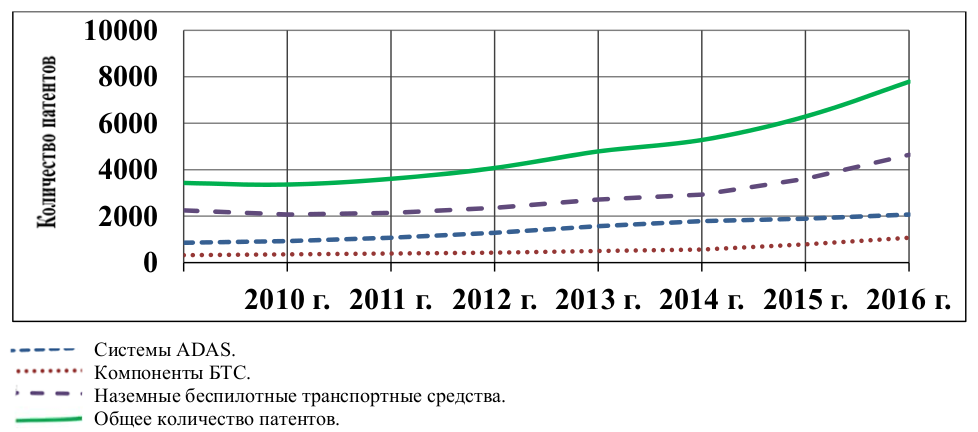
\includegraphics[scale=0.5]{views/patent.png}
    }
    \caption{Динамика патентования за рубежом наземных беспилотных транспортных средств, систем ADAS и компонентов БТС в целом и раздельно за период с 2010 по 2016 годы}\label{fig:patent}
\end{figure}

Для реализации автономного управления движением беспилотного транспортного средства наиболее активно ведутся разработки и патентуются системы управления движением БТС, которые включают: блоки управления интеллектуальным шасси, системы технического зрения, обработки и передачи информации, системы навигации и ориентации (рисунок~\cref{fig:system}). 

\begin{figure}[ht]
    \centerfloat{
        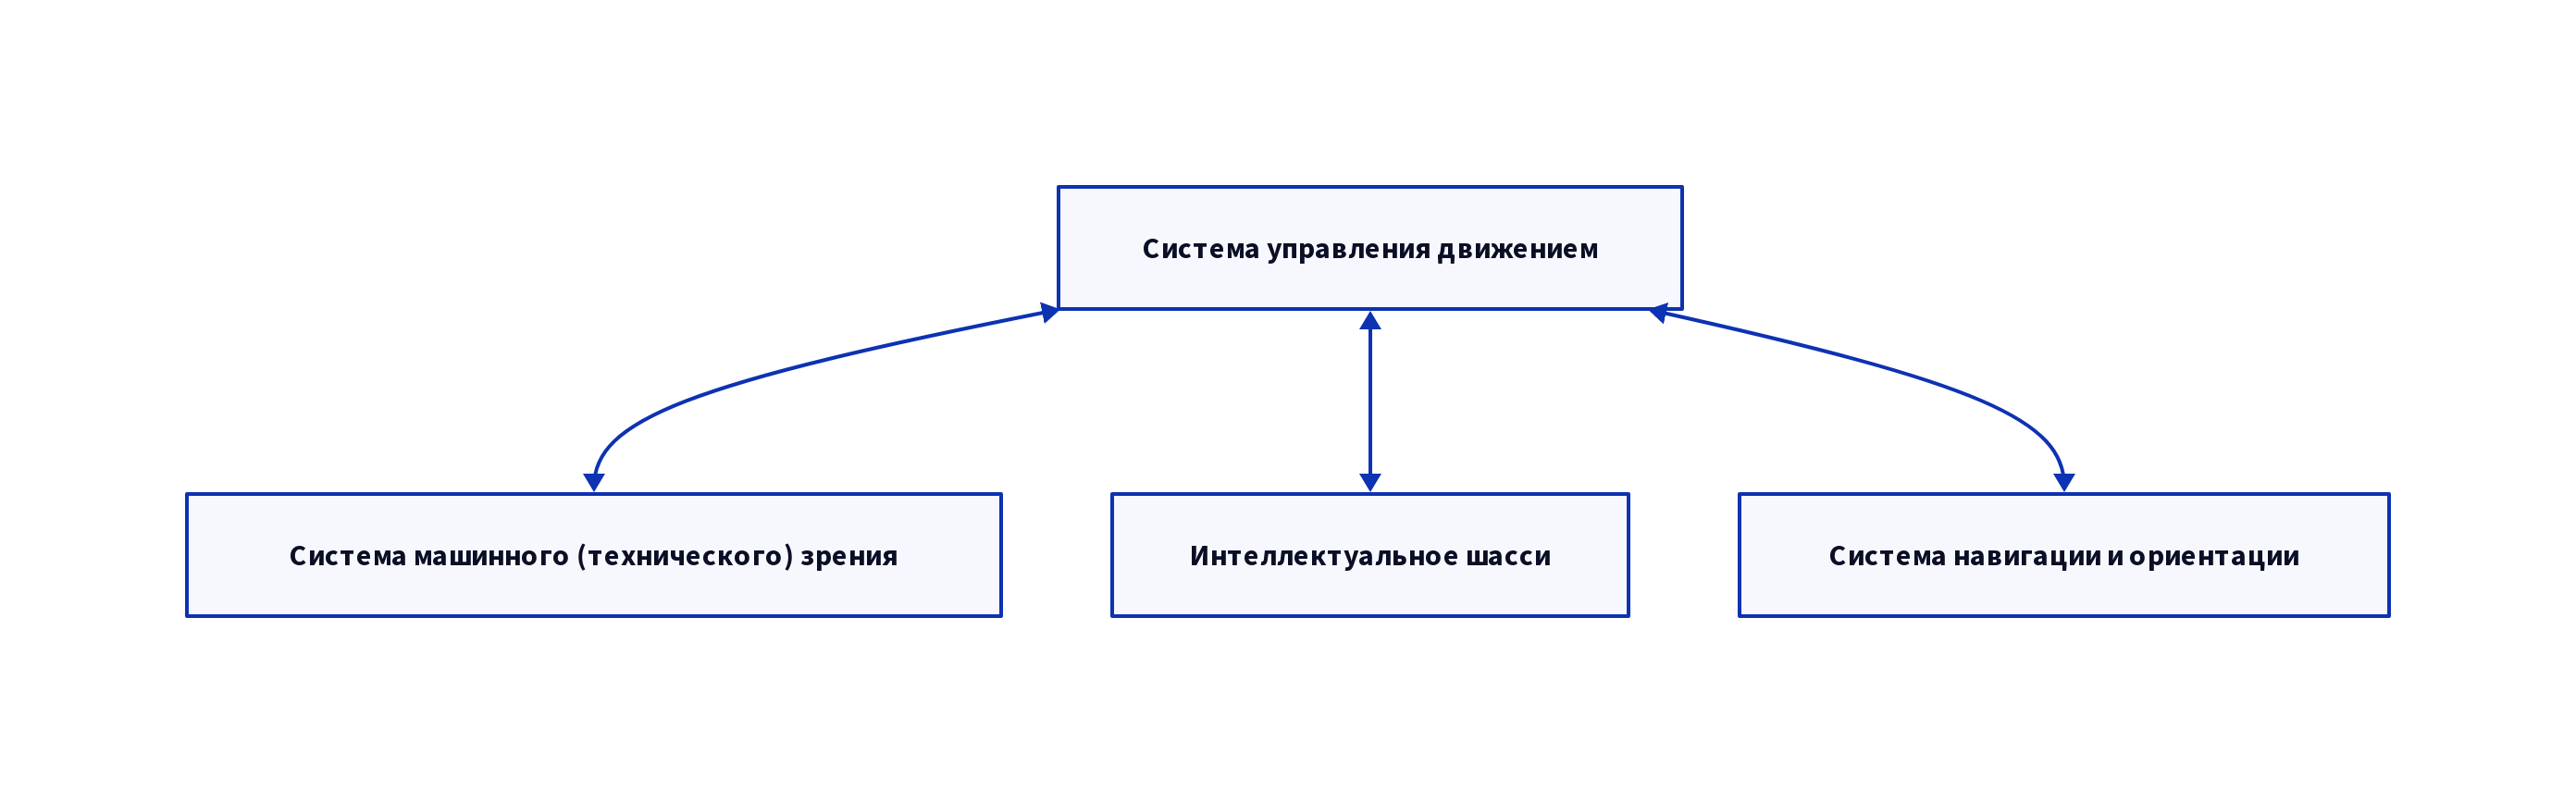
\includegraphics[scale=0.2]{d2/system.png}
    }
    \caption{Подсистемы автоматизированной системы управления БТС}\label{fig:system}
\end{figure}


Конкретным примером в сфере НТТС можно рассмотреть разработку Научно-технического центра ПАО «КАМАЗ» совместно со специалистами МГТУ им. Н. Э. Баумана: самосвал КАМАЗ-6559 (рисунок~\cref{fig:ypiter30}), предназначенный для карьерных работ в автономном режиме.

\begin{figure}[ht]
    \centerfloat{
        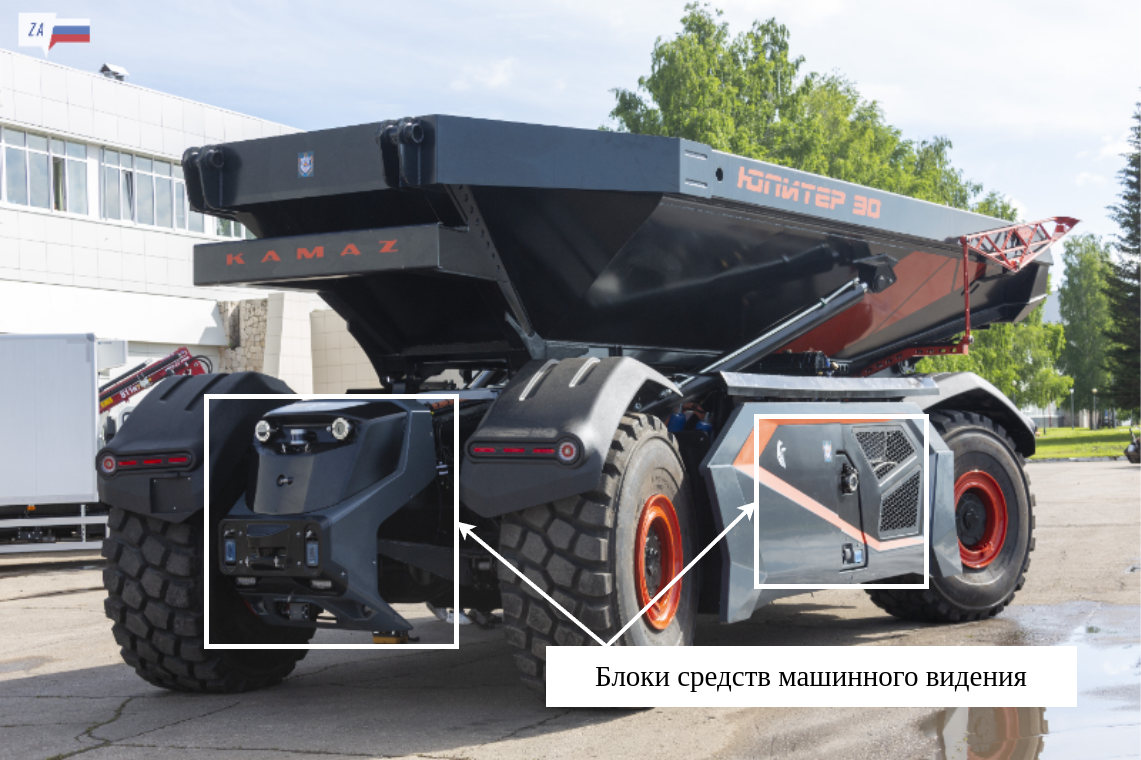
\includegraphics[scale=0.1]{views/kamaz.jpg}
    }
    \caption{Беспилотный КАМАЗ-6559 («Юпитер 30»)}\label{fig:ypiter30}
\end{figure}

Самосвал создан в рамках проекта «Создание семейства электромеханических беспилотных автомобилей-самосвалов большой грузоподъёмности в интересах добывающих отраслей промышленности РФ». Предназначен для перевозки разрыхлённой горной массы или руды по безлюдной технологии – без присутствия людей в опасной зоне работы большегрузных машин и экскаваторов. В связи с этой особенностью в конструкции автомобиля отсутствует кабина для водителя. НТТС изначально проектировался как автономное транспортное средство для работы в карьере. В нём установлены специальные, защищённые от пыли, грязи, влаги и вибраций видеокамеры, 2D- и 3D-лидары, ультразвуковые датчики, радары. Также имеются GSM-антенны и GPS/ГЛОНАСС навигация.

\section{Основные принципы автоматизации процесса работы НТТС}\label{sec:ch1/sec2}

В общем виде системы управления движением БТС обеспечивают выполнение следующих операций:

\begin{itemize}
    \item получение и обработку данных с датчиков;
    \item объединение и согласование полученных данных;
    \item обработку изображений;
    \item определение препятствий, дорожных условий и автомобилей, расстояния до них;
    \item позиционирование БТС и определение текущего состояния системы;
    - реализацию автоматического управления скоростью БТС, траекторией (курсом) движения, автоматической реакцией на объекты, окружающие БТС;
    \item принятие решений на управляющие действия;
    \item управление исполнительными устройствами;
    \item формирование базы данных для последующего анализа.
\end{itemize}

\subsection{Системы управления и контроля}\label{subsec:ch1/sec2/sub1}

По степени автоматизации различают машины с механизированным управлением, с автоматизированным управлением и контролем на базе микропроцессорной техники, с автоматизированным управлением на расстоянии, с автоматическим управлением на базе микропроцессоров и мини-ЭВМ, строительные манипуляторы и роботы, а также роботизированные машины и комплексы \cite[с.~39]{Evtukov}.

Системы управления предназначены для включения и выключения различных механизмов машин \cite[с.~109]{Evtukov}.
По назначению системы управления можно разделить на следующие: управлением двигателем; управление муфтами и тормозами; рулевое управление; управление рабочим органом (например, опускание и подъем отвала бульдозера или ковша скрепера, поворот отвала автогрейдера).

По конструкции системы управления строительных машин разделяют на механические, гидравлические, пневматические, электрические и смешанные (комбинированные), аналогично силовым приводам, но в отличие от которых в большинстве случаев в системах управления передаются значительно меньше силы.

Различают машины с механизированным и автоматизированным управлением. Автоматизированное управление и контроль рабочего процесса могут осуществляться на базе микропроцессоров и мини-ЭВМ, а также строительные манипуляторы и роботы, роботизированные машины и комплексы.

\subsection{Использование датчиков и сенсоров}\label{subsec:ch1/sec2/sub2}

С помощью различных датчиков обеспечивается сбор данных о состоянии окружающей среды. Датчики можно классифицировать на датчики внешней информации и внутренней \cite[с.~131]{Vlasov}. 

Датчики внутренней информации представляют собой в основном преобразователи механических параметров в электрические сигналы. Например датчики обратной связи по положению, скорости и ускорения.

\begin{figure}[ht]
    \centerfloat{
        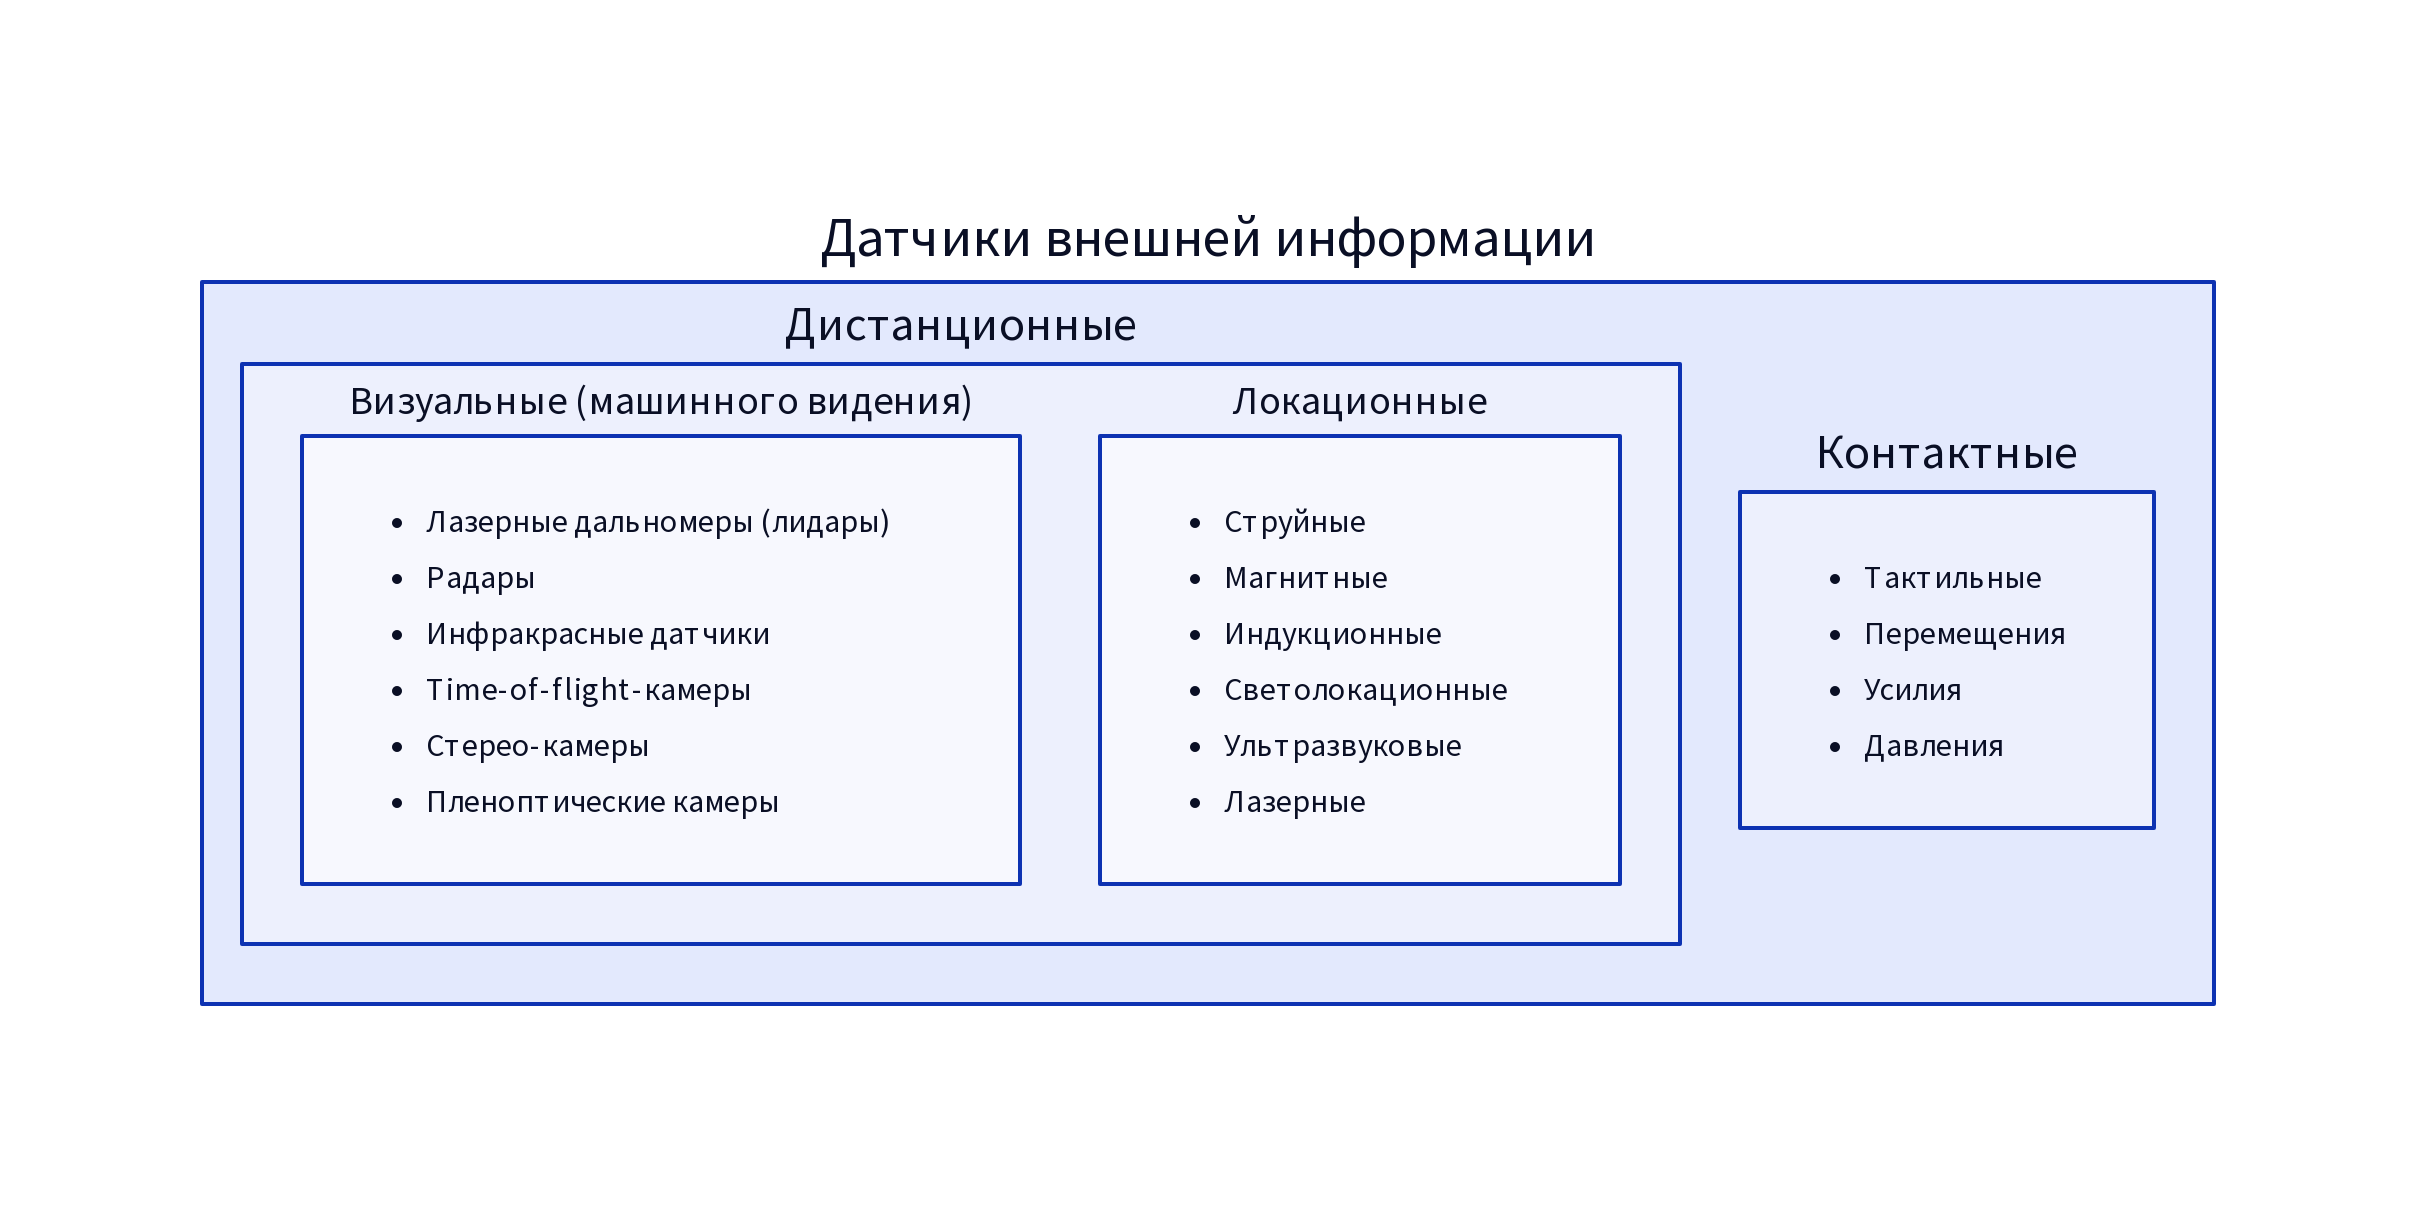
\includegraphics[scale=0.2]{d2/datchiki}
    }
    \caption{Классификация датчиков внешней информации}\label{fig:datchiki}
\end{figure}

Датчики внешней информации обеспечивают сбор информации об окружающем мире. Их можно разделить на две большие группы (рис.~\cref{fig:datchiki}): дистанционные и контактные. В свою очередь дистанционные датчики можно разделить на локационные и визуальные.

Локационные системы можно условно разделить на два класса: дальней и ближней локации. Первые могут быть построены с использованием ультразвуковых, лазерных и светолокационных датчиков.

Визуальные системы (технического, машинного зрения) относятся к числу наиболее сложных, но и наиболее универсальных средств очувствления НТТС (рис.~\cref{fig:kamaz},~\cref{fig:robot1},~\cref{fig:robot2},~\cref{fig:sensors}).

\begin{figure}[ht]
    \centerfloat{
        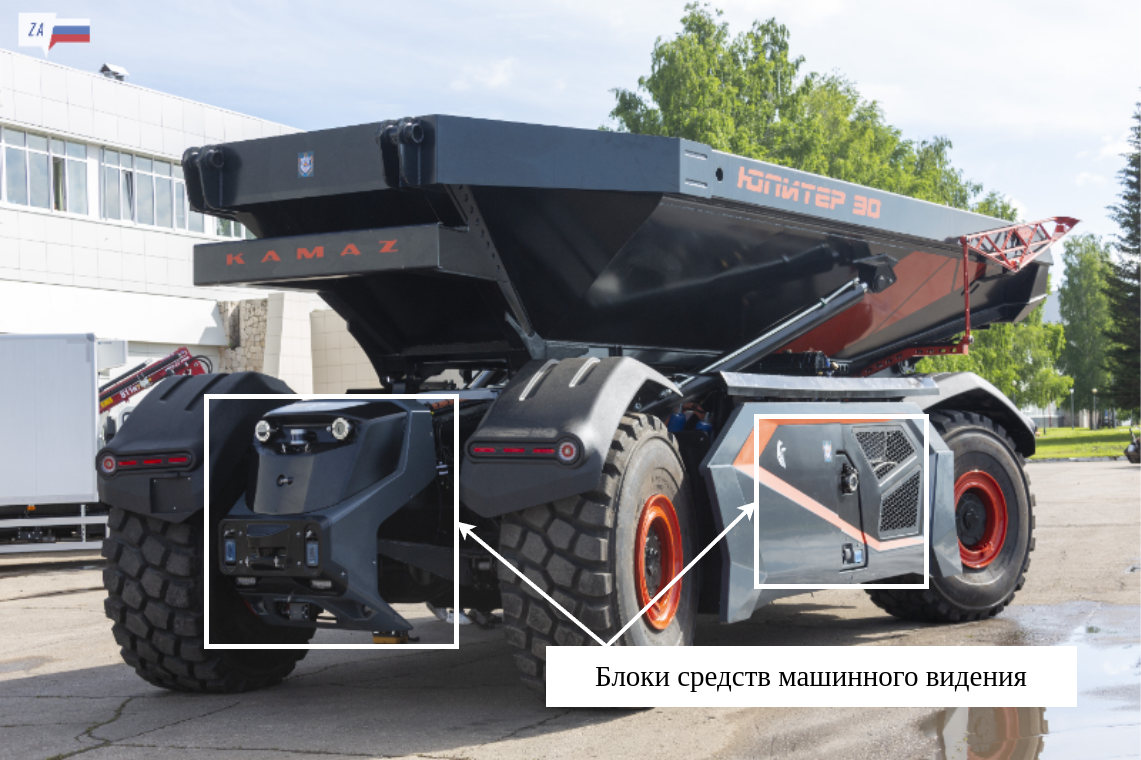
\includegraphics[scale=0.2]{views/kamaz.png}
    }
    \caption{Набор датчиков «Юпитер-30» ПАО «КАМАЗ»}\label{fig:kamaz}
\end{figure}

\begin{figure}[ht]
    \centerfloat{
        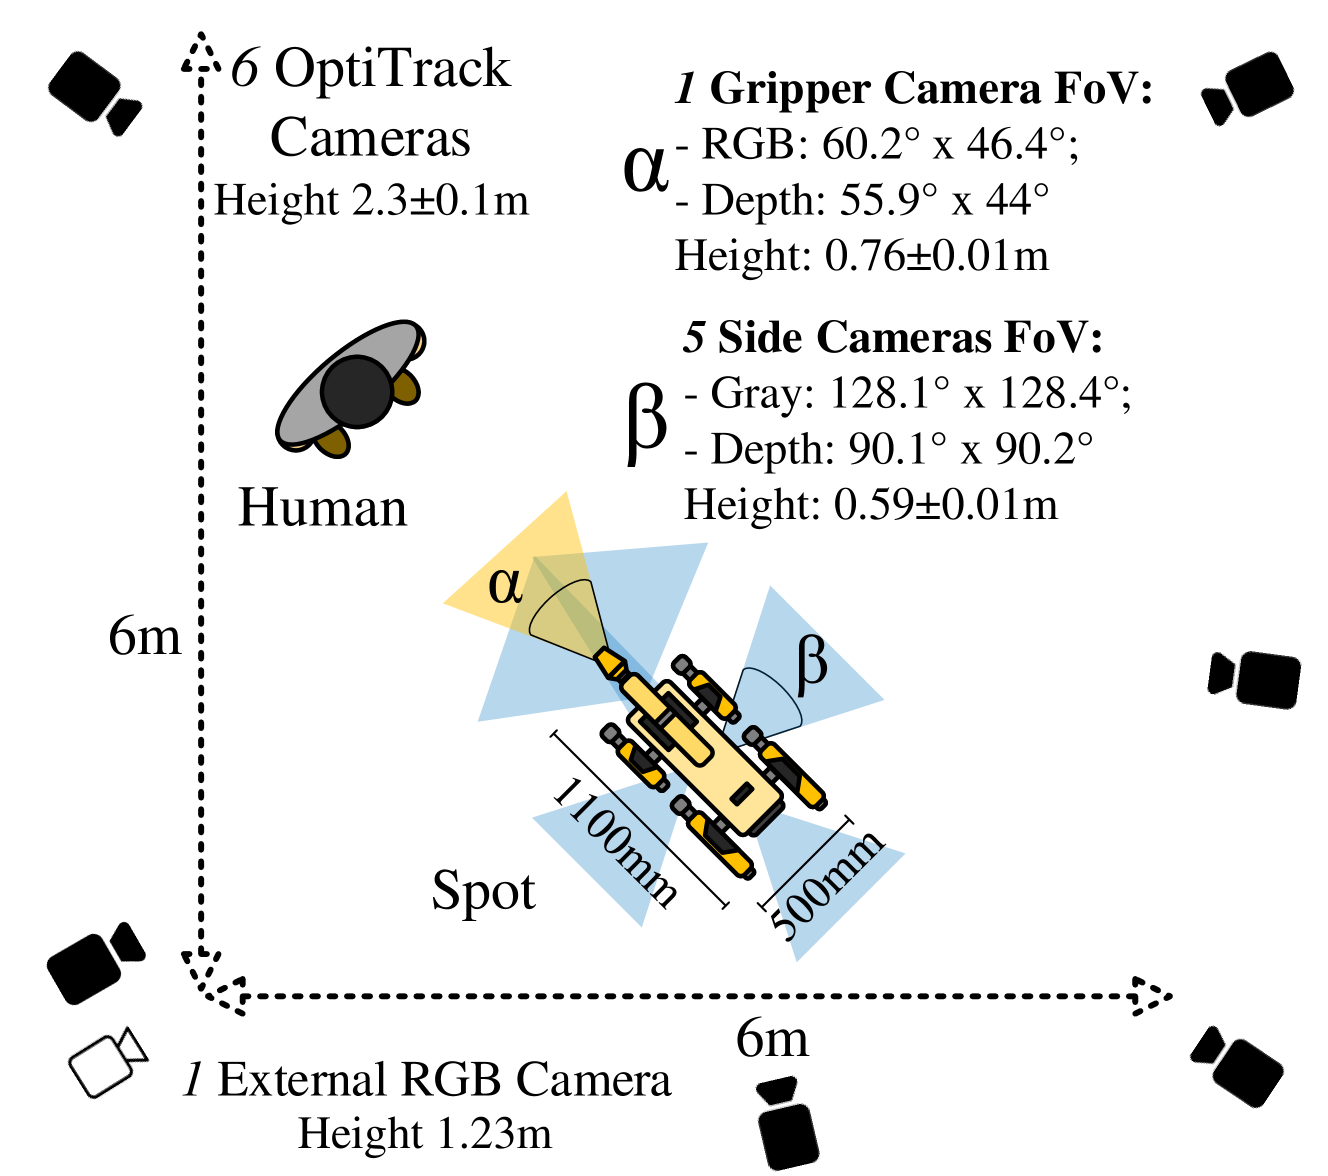
\includegraphics[scale=0.2]{views/robot1.png}
    }
    \caption{Набор датчиков автономного робота}\label{fig:robot1}
\end{figure}

\begin{figure}[ht]
    \centerfloat{
        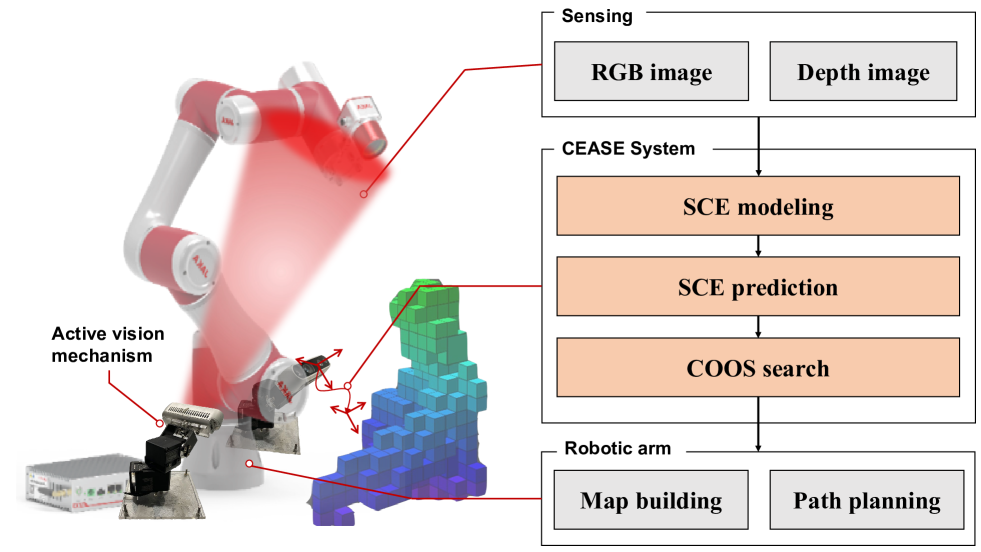
\includegraphics[scale=0.2]{views/robot2.png}
    }
    \caption{Набор датчиков робота}\label{fig:robot2}
\end{figure}

\begin{figure}[ht]
    \centerfloat{
        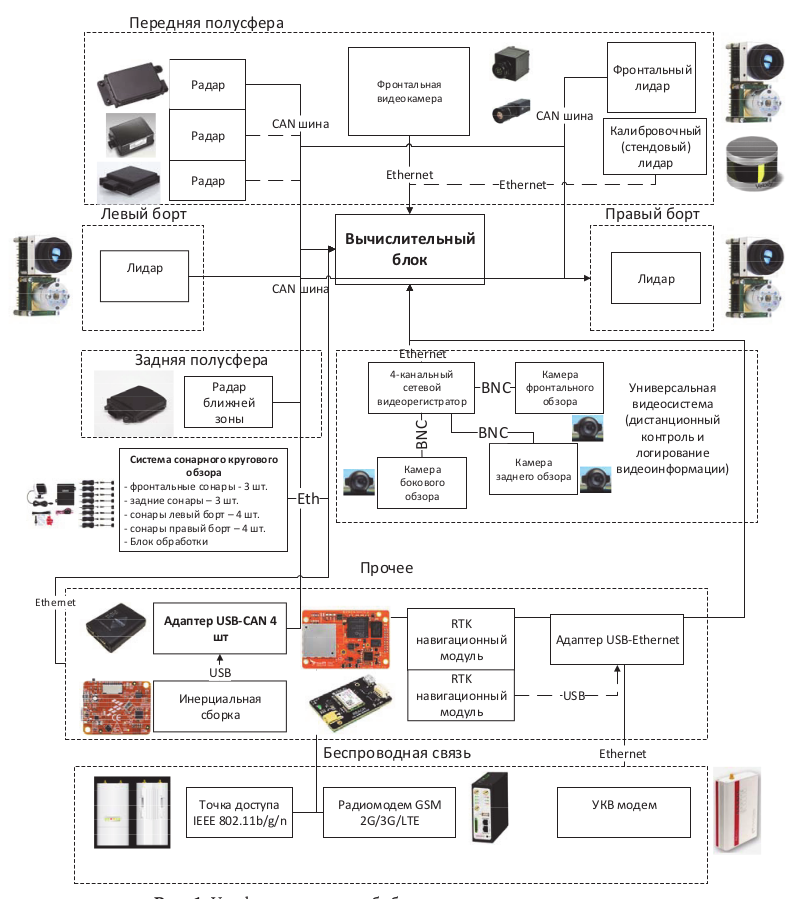
\includegraphics[scale=0.6]{views/sensors.png}
    }
    \caption{Унифицированная схема взаимосвязи датчиков}\label{fig:sensors}
\end{figure}


Основными~\cite{confbib1} используемыми средствами машинного видения являются:

Лазерные дальномеры (лидары), которые измеряют расстояние до объектов. Результат работы лидара – объемная сцена из облака точек с геометрией объектов. Это средство выдает наибольшую точность, лучше всех работают на ровных поверхностях и почти не засвечиваются солнцем. При этом имеют высокое энергопотребление, относительно низкую частоту кадров, бегущий затвор и необходимость компенсировать его при обработке, а также работающие рядом лидары создают друг-другу помехи, которые не так просто компенсировать.

Радары для определения расстояния до объекта, его скорости и месторасположения. Радары меньше зависят от погоды и стоят намного дешевле лидаров. Главным отрицательным качеством является то, что плохо обнаруживаются неметаллические объекты, в том числе пешеходы.

Инфракрасные датчики для реагирования на фоновое инфракрасное излучение. Прибор регистрирует любое тепловое излучение.

Time-of-flight-камеры (ToF\nomenclature{ToF}{Time-of-flight-камеры\nomrefpage}) - видеокамеры, формирующие дальностное изображение. Используются для создания изображений, которые в качестве пикселей содержат оценки расстояний от экрана до конкретных точек наблюдения.

Стерео-камеры, построенные на имитации бинокулярного зрения человека с возможностью захватывать трехмерные изображения.

Пленоптические камеры, фиксирующие векторное поле световых лучей (световое поле). На основе картины светового поля может быть воссоздана наиболее полная информация об изображении, пригодная для решения различных задач компьютерной графики.

Обычные камеры с последующим анализом видео-потока с применением алгоритмов машинного обучения.

Так же можно приобщить разрабатываемый метод обмена данными о местоположении, скорости, направлении движения и другими данными между объектами.

Одновременно с этим, применение какого-либо одного средства недостаточно, так как получение комплексного видения окружающего мира роботами имеет сложности в виде:

\begin{itemize}
    \item темного времени суток;
    \item засветов от солнца и источников освещения;
    \item инфракрасного излучение солнечного света;
    \item осадков и грязи;
    \item множественности и вариативности подвижных окружающих объектов.
\end{itemize}

В связи с этим, средства машинного видения применяются комплексно, для компенсации недостатков друг-друга. Сравнительный анализ приведен в~таблице~\ref{tab:TableViews}.

\begin{table}[htbp]
    \centering
    \begin{threeparttable}
        \caption{Сравнительный анализ средств машинного видения}\label{tab:TableViews}%
            \begin{tabular}{{| p{3cm} || p{2cm} | p{2cm} | p{2cm} | p{2cm} | p{2cm} |}}
            \hline
            & ToF & Стерео & Пленопт. & Лидары & Радары \\ \hline
            Разрешение                 & \textit{Слабо}  & Средне & \textbf{\begin{tabular}[c]{@{}l@{}}Отлично\\ (сцена)\end{tabular}} & \begin{tabular}[c]{@{}l@{}}Средне\\ (сцена)\end{tabular} & \textit{Слабо}  \\ \hline
            Точность                    & Средне          & Средне          & \textit{Слабо}            & \textit{Слабо}  & \textbf{Высоко} \\ \hline
            Сложность ПО \nomenclature{ПО}{программное обеспечение\nomrefpage}                & \textbf{Слабо}  & Средне          & \textit{Высоко}           & \textit{Высоко} & \textbf{Слабо}  \\ \hline
            Работа в реальном времени   & \textbf{Высоко} & Средне          & Средне                    & Средне          & \textit{Слабо}  \\ \hline
            Стоимость                   & Средне          & Средне          & \textbf{Слабо}            & \textit{Высоко} & Средне          \\ \hline
            Производ-сть при слабом освещении & \textbf{Хорошо} & \textbf{Хорошо} & \textit{Плохо}            & \textit{Плохо}  & \textbf{Хорошо} \\ \hline
            Работа на открытом воздухе  & \textit{Плохо}  & \textit{Плохо}  & \textbf{Хорошо}           & \textbf{Хорошо} & \textbf{Хорошо} \\ \hline
            \end{tabular}
    \end{threeparttable}
\end{table}

Можно сделать вывод, что по разрешению лидируют пленоптические камеры, но все очень сильно зависит от сцены. По точности - лидары. По сложности обработки - «непосредственно» получают глубину только ToF и лидары. По частоте кадров конструктивно хороши ToF-камеры. При работе на открытом пространстве плохо работают ToF и камеры структурированного света.

Однозначно стоит в дальнейшем изучить и проанализировать использование совместно со средствами машинного видения такие методы, как:

\begin{itemize}
    \item определение местоположения в пространстве на основе глобальных систем позиционирования (GPS, ГЛОНАСС);
    \item получение данных от коллекторов навигационных данных (системы типа Яндекс-навигатор);
    \item заранее заложенные геопространственные данные;
    \item передачу управляющих сигналов внешними специализированными автоматизированными системами управления (по анализу данных с наружных камер наблюдения, управляющее воздействие регулятора и т.д.).
\end{itemize}


\subsection{Программное обеспечение для автоматизации}\label{subsec:ch1/sec2/sub3}

Программное обеспечение для автоматизации

\section{Координация автоматизированных НТТС}\label{sec:ch1/sec3}

Координация автоматизированных наземных транспортно-технологических средств

\section{Выводы по главе}\label{sec:ch1/sec4}

Выводы

\FloatBarrier
           % Глава 1
\chapter{Моделирование координации автоматизированных наземных транспортно-технологических средств}\label{ch:ch2}

\section{Модель системы многозадачной координации АНТТС}\label{sec:ch2/sec1}

Модель системы многозадачной координации автоматизированных наземных транспортно-технологических средств (АНТТС\nomenclature{АНТТС}{автоматизированные наземные транспортно-технологические средства\nomrefpage}).

\section{Рациональное планирование ресурсов для многозадачной координации АНТТС}\label{sec:ch2/sec2}

Рациональное планирование ресурсов для многозадачной координации автоматизированных наземных транспортно-технологических средств.

\section{Выводы по главе}\label{sec:ch2/sec3}

Выводы

\FloatBarrier
           % Глава 2
\chapter{Моделирование и оптимизация}\label{ch:ch3}

\section{Моделирование различных сценариев работы}\label{sec:ch3/sec1}

Некоторый текст.

\section{Проведение симуляций для оценки производительности}\label{sec:ch3/sec2}

Некоторый текст.

\section{Оптимизация рабочего процесса и координации задач}\label{sec:ch3/sec3}

Некоторый текст.

\FloatBarrier           % Глава 3
\chapter{Экспериментальные исследования и оценка результатов}\label{ch:ch4}

\section{Описание экспериментальной симуляционной среды}\label{sec:ch4/sec1}

Некоторый текст.

\section{Проведение тестов на симуляционных данных}\label{sec:ch4/sec2}

Некоторый текст.

\section{Сравнительный анализ результатов с существующими методами}\label{sec:ch4/sec3}

Некоторый текст.

\FloatBarrier           % Глава 4
\chapter{Практическая реализация и внедрение}\label{ch:ch5}

\section{Возможности применения разработанного метода на практике}\label{sec:ch5/sec1}

Некоторый текст.

\section{Описание потенциальных областей внедрения}\label{sec:ch5/sec2}

Некоторый текст.

\section{Рекомендации по внедрению на базе предложенного метода}\label{sec:ch5/sec3}

Некоторый текст.

\FloatBarrier           % Глава 5
\chapter*{Заключение}                       % Заголовок
\addcontentsline{toc}{chapter}{Заключение}  % Добавляем его в оглавление

%% Согласно ГОСТ Р 7.0.11-2011:
%% 5.3.3 В заключении диссертации излагают итоги выполненного исследования, рекомендации, перспективы дальнейшей разработки темы.
%% 9.2.3 В заключении автореферата диссертации излагают итоги данного исследования, рекомендации и перспективы дальнейшей разработки темы.
%% Поэтому имеет смысл сделать эту часть общей и загрузить из одного файла в автореферат и в диссертацию:

Основные результаты работы заключаются в следующем.
\input{common/concl}

В заключение автор 
      % Заключение
\include{Dissertation/acronyms}        % Список сокращений и условных обозначений
\chapter*{Словарь терминов}             % Заголовок
\addcontentsline{toc}{chapter}{Словарь терминов}  % Добавляем его в оглавление

\textbf{ADAS} : Advanced Driver-Assistance Systems, усовершенствованная система помощи водителю       % Словарь терминов
\include{Dissertation/references}      % Список литературы
\include{Dissertation/lists}           % Списки таблиц и изображений (иллюстративный материал)

\setcounter{totalchapter}{\value{chapter}} % Подсчёт количества глав

%%% Настройки для приложений
\appendix
% Оформление заголовков приложений ближе к ГОСТ:
\setlength{\midchapskip}{20pt}
\renewcommand*{\afterchapternum}{\par\nobreak\vskip \midchapskip}
\renewcommand\thechapter{\Asbuk{chapter}} % Чтобы приложения русскими буквами нумеровались

\chapter{Приложение}\label{app:A}

\section{Подраздел приложения}\label{app:A1}

\clearpage
        % Приложения

\setcounter{totalappendix}{\value{chapter}} % Подсчёт количества приложений

\end{document}
